\documentclass{article}
\usepackage{graphicx}
\usepackage{hyperref}
\usepackage{multicol}
\usepackage{amssymb}
\usepackage{titlesec}
\usepackage{eurosym}
\usepackage{listings}
\usepackage{xcolor}

\colorlet{punct}{red!60!black}
\definecolor{background}{HTML}{EEEEEE}
\definecolor{delim}{RGB}{20,105,176}
\colorlet{numb}{magenta!60!black}

\lstdefinelanguage{json}{
    basicstyle=\normalfont\ttfamily,
    numbers=left,
    numberstyle=\scriptsize,
    stepnumber=1,
    numbersep=8pt,
    showstringspaces=false,
    breaklines=true,
    frame=lines,
    backgroundcolor=\color{background},
}

\titleclass{\subsubsubsection}{straight}[\subsection] 

\newcounter{subsubsubsection}[subsubsection]
\renewcommand\thesubsubsubsection{\thesubsubsection.\arabic{subsubsubsection}}
\renewcommand\theparagraph{\thesubsubsubsection.\arabic{paragraph}} % optional; useful if paragraphs are to be numbered

\titleformat{\subsubsubsection}
  {\normalfont\normalsize\bfseries}{\thesubsubsubsection}{1em}{}
\titlespacing*{\subsubsubsection}
{0pt}{3.25ex plus 1ex minus .2ex}{1.5ex plus .2ex}

\makeatletter
\renewcommand\paragraph{\@startsection{paragraph}{5}{\z@}%
  {3.25ex \@plus1ex \@minus.2ex}%
  {-1em}%
  {\normalfont\normalsize\bfseries}}
\renewcommand\subparagraph{\@startsection{subparagraph}{6}{\parindent}%
  {3.25ex \@plus1ex \@minus .2ex}% chktex 1
  {-1em}%
  {\normalfont\normalsize\bfseries}}
\def\toclevel@subsubsubsection{4}
\def\toclevel@paragraph{5}
\def\toclevel@paragraph{6}
\def\l@subsubsubsection{\@dottedtocline{4}{7em}{4em}}
\def\l@paragraph{\@dottedtocline{5}{10em}{5em}}
\def\l@subparagraph{\@dottedtocline{6}{14em}{6em}}
\makeatother

\setcounter{secnumdepth}{4}
\setcounter{tocdepth}{4}

\newcounter{choice}
\renewcommand\thechoice{\Alph{choice}}
\newcommand\choicelabel{\thechoice.}

\newenvironment{nielsenenumerate}
{ \begin{enumerate}
    \setlength{\itemsep}{4pt}
    \setlength{\parskip}{0pt}
    \setlength{\parsep}{0pt}     }
{ \end{enumerate}                  } 

\newenvironment{myenumerate}
{ \begin{enumerate}
    \setlength{\itemsep}{0pt}
    \setlength{\parskip}{0pt}
    \setlength{\parsep}{0pt}     }
{ \end{enumerate}                  } 

\newenvironment{myitemize}
{ \begin{itemize}
	\setlength{\itemsep}{0pt}
    \setlength{\parskip}{0pt}
    \setlength{\parsep}{0pt}     }
{ \end{itemize}                  } 

\newcommand\tabsmall[1][0.8cm]{\hspace*{#1}}
\newcommand\tab[1][3cm]{\hspace*{#1}}

\begin{document}
    
\begin{titlepage}
    \centering
    
    
    
\includegraphics[scale=0.5]{chapters/title_page/logo_uhasselt}		
    \vspace{1cm}
    
    \Huge The Modular Electronic Health Record Dashboard: A Novel Approach to Interoperability and Usability
    \vspace{0.4cm}
    
    \large Master thesis Computer Science
    \vspace{1cm}
    
    \LARGE Dennis Cardinaels
    \vspace{1cm}
    
    \large Promotor: Professor Mieke Haesen
    \vspace{0.2cm}
    
    Assistant: Jens Brulmans
    
    \vspace{1.2cm}
    
    
    \Large 2018 -- 2019 % chktex 8
    
\end{titlepage}

	\pagenumbering{roman}
	
	\section*{Acknowledgements}
\addcontentsline{toc}{section}{Acknowledgements}

This thesis was the largest challenge I faced in my academic career. Throughout the entire process I expanded my knowledge in the health informatics domain greatly. The end result of this thesis would not have been possible without the support of the following people:
\begin{itemize}
    \item Professor Mieke Haesen and Jens Brulmans. Whenever I had questions or uncertainties, I could reach out to them for feedback and I am grateful for their guidance.
    \item The test participants that volunteered to participate in the usability test.
    \item My parents for their continued support through thick and thin.
    \item My close friends and roommates to provide me with the occasional rest and recreation.
\end{itemize}
	
    \section*{Abstract}
\addcontentsline{toc}{section}{Abstract}

TODO

    
    \tableofcontents
	\newpage
    \pagenumbering{arabic}
    
    \section{Introduction}

With the continuous growth of ubiquitous computing, the possibility of continuing rehabilitation at home rises. The caregiver monitors the patient at a distance and if needed, the patient is contacted. As a result, resources on both the caregiver and patient side can be saved. This process is called telemonitoring. Research investigated telemonitoring for chronic disease management. Due to the length of these conditions, patients report the status of their condition using a device such as a smartphone or digital blood pressure monitor.

New platforms are created by telemonitoring literature, instead of reusing one or extending an existing health system. Using different applications to monitor for example diabetes and cardiovascular diseases would result in redundancy, as parameters such as blood pressure are important for both disease groups. These values need to be updated at two locations, which leads to higher chance of human error. The ability to monitor all parameters in one singular location, would prove to be beneficial.

Most health care institutions have transitioned to electronic patient records. Software solutions interact with these records to automatically generate statistics, decision support, and many types of alerts. Monolithic software applications are often used for more general care, while specific software applies to specific types of care. There are benefits and drawbacks to both, but no literature was found which reported on integrating the specific applications with a monolithic system. In a perfect world, one singular system provides all the required functionality.

Another gap in health software research, is the effect of customization. Each patient is different and a customized rehabilitation trajectory is preferred. Current health systems provide a general view for all patients, where relevant information is buried behind many different screens and menus. Should the software allow the clinicians to indicate what is of importance, this information can be reached much faster. In other words, a customized dashboard gathers all important data as indicated by the caregiver in a singular location. This dashboard can generate summaries, while details are one click away. 

The issues mentioned in the last few paragraphs signify the need to quickly see relevant information at a glance. Not only for telemonitoring, but also for general care given in a hospital setting, this can be beneficial. Together with customization, care is delivered with greater efficiency. This thesis proposes a dashboard design that allows the caregiver to personalize its functionality according to the patient's needs in terms of treatment. It will mainly focus on chronic disease management for use in telemonitoring.

First, to get a thorough understanding of related subjects, a background information is given in section \ref{background}. The topics include electronic health record systems, chronic disease management, a literature review on telemonitoring, dashboard design, and health data privacy and standards. Based on this background information a dashboard design is proposed (section \ref{design}). This section highlights the design process and the made choices. Also, personas, scenarios and paper mockups give a first indication of how the system is used. Implementation of the dashboard started after the design process. In section \ref{implementation} the used frameworks and changes compared to the low fidelity prototypes are described.

As soon as the implementation was finished, a usability test was conducted. Section \ref{usabilitytest} describes the test setup, the created documents, and information concerning the testers. The results of the test are discussed in the following section. Finally, the thesis concludes with a summary of its findings. 
	
	\section{Background} \label{background}

A literature study has been conducted to situate the thesis topic. Multiple subjects lay at the base of the design mentioned in section \ref{design}. Because this design describes a health platform, a general overview of electronic health record systems is given first. The precise topics are the transition to, the components of, and the types of these systems. Next three key subjects are explained in the following order: chronic diseases, telemonitoring, and dashboard design. The last section briefly mentions the issues surrounding medical data privacy and standards. 

    % waarom belangrijk om te beschrijven
    \subsection{Electronic health record systems}

    Health information systems are becoming an important part of health care. They support patient care as well as administrative and financial tools. At the heart of these systems lies the electronic health record. An electronic health record (EHR) is a repository of electronically maintained information about an individual's health status and health care, stored such that it can serve multiple legitimate uses and users of the record \cite{biomedical_informatics}. An electronic health record system (EHRS) provides tools to manage and interact with these records. These tools include reminder generation, data analysis, and decision support. It helps the clinician to organize, interpret and react to medical data.

    The first section describes the transition from paper-based records to digital and its implications for the medical world. A summary of the main components present in an EHRS is described in the next section. The functionality of an EHRS can be categorized into two types: a monolithic system tries to provide more general care, while smaller and more specialized systems cater to more specific types of care. The last section compares the two types and highlights the benefits and drawbacks of both.

    No existing EHRS were reviewed. Access to these systems is limited to open-source solutions as most are commercial and sometimes off-the-shelf products. Consequently, reviews of these systems are difficult to find as institutions only purchase software after thorough review of its features. Only one article was found which compared three open-source health systems \cite{de2012overview}. However, no literature was found for proprietary systems.

        % signify importance
        \subsubsection{Moving away from paper} \label{2_ehrs_paper}

        For modern medicine, traditional paper-based medical records are not suited for today's world filled with technology. The drawbacks of information on paper are obvious when compared to digitally stored information.

        \paragraph{Functionality} Digital records allow systems to aggregate, process and create statistics of the data it contains. For example, a system can generate heart rate graphs with statistics, summarizing many values. If the user hovers over a data point in the graph, the exact value is shown. Printed tables and graphs showing the same data lack this interaction. Also, paper records demand more effort from clinicians as data is often spread across multiple dossiers.

        A paper-based medical dossier can store for example medical images, such as x-rays. Compared to a digital image, paper loses a lot of detail. As such, most multimedia types can only be stored digitally and not on paper. Tools to interact with these file types are provided by an EHRS.

        In terms of data input, an EHRS can detect and prevent false data input. The system ensures that all necessary data fields are filled in and in the correct format. This results in more complete and accurate data gathering with fewer errors, increasing the information quality.

        \paragraph{Information quality} A summarizing paper noted that the use of EHRS leads to more complete, accurate, comprehensive, and reliable data compared to paper-based records \cite{ehrs_summary}. As mentioned in the previous paragraph, a digital system can impose rules on data fields to avoid missing or entering the wrong data. In terms of comprehensibility, poor handwriting leads to wrong or loss of information, which digital systems avoid. Medical instruments can save measurements immediately into system, avoiding copying by hand.

        \paragraph{Accessibility} Paper records are difficult to access because most of the time only one copy exists. Therefore, transferring these records to other branches or institutions is difficult as the record needs to be located in the often large medical dossier. Also, misfiling, flooding or fires lead to irrecoverable loss of the data. Creating backups of the digital records avoids the last issue, but difficulties surrounding data transfer are still present. Most institutions have their own database structures which hinders the transfer of raw medical data. To remedy this, interfaces are created by the IT staff to interpret and store the data. Sending for example PDF-reports via email is a convenient alternative, although limited in functionality comparable to an actual paper record. Therefore, integration capabilities and the use of standards (section \ref{2_privacy}) are important for an EHRS. 

        Moving data from paper to a digital format requires a lot of manual work. While automation is possible, such as scanning and processing the paper forms with software, verification is still necessary. All the data fields from the documents need to find a place in the system, which is difficult to achieve. Extra diagnostic information scribbled all over the the document, will be lost during this process. Also, what do we do with unreadable data due to poor handwriting? What happens with two forms which contain partly the same information? Do we save the information twice or do we add extra checks to prevent duplication? Because of these reasons, adopting an EHRS is a significant undertaking for an institution. As such, the benefits are not immediately apparent.

        Because digital storage increases accessibility significantly, security measurements have to be taken. If not, data can be stolen, deleted or even altered, which means a breach of privacy (section \ref{2_privacy}). This also adds to the complexity of developing EHRS. 

        \paragraph{Efficiency} An important task of an EHRS is to facilitate effective care. An early study saw a 6\% increase in productivity when EHRS were deployed in health care institutions \cite{ehrs_efficiency}. However, other factors are at play, such as the adoption rate. The transition from paper-based documenting to digital is accompanied by a learning curve, which can be steep. After the switch, the productivity will most likely be lower at the start. As the users become more experienced with the software, it will increase. Today most institutions have already made the transition to an EHRS, so this has become less of an issue.

        \subsubsection{Components of an EHRS} \label{ehrs_components}

        As mentioned before, EHRS do not simply store patient records. They consist of many components which ultimately defines how well they perform in health care. Literature defines many lists of essential components. However, we define the following five components as key \cite{biomedical_informatics}:

        \paragraph{Integrated view of patient data} An EHR must allow storage of a wide range of data types. This can be text, numbers, images, video, and others. Some data can still be on paper due to lacking support of the EHRS, as mentioned in section \ref{2_ehrs_paper}. To display more complex data types, such as x-ray images, standards are used. A brief overview of medical standards is described in section \ref{2_standards}.

        \paragraph{Clinician order entry} The point at which the clinician enters treatment instructions is called order entry. An order entry system assists the clinician during the decision-making process to ensure that the instructions are correct. It also reduces errors and costs compared to paper order entry for the same reasons already mentioned in section \ref{2_ehrs_paper}.

        \paragraph{Clinical decision support} A decision support system embed into an EHRS aids the clinician by suggesting certain actions when certain situations occur. If for example, a patient is due for vaccination, the system notifies the clinician by presenting a constructed order which needs to be confirmed or denied. The system can do this for a bulk of patients, so manual checkups are not required, thus saving time.

        \paragraph{Access to knowledge resources} During the writing of notes or orders for a patient, clinical questions often arise. Instead of asking colleagues or searching through multiple manuals, the EHRS searches for relevant literature to address the question. Due to the internet, a very large source of information is readily available.

        \paragraph{Integrated communication and reporting support} Communication is an important part of health care. Often clinicians spread across multiple institutions provide care for the same patient. Communication, therefore, directly affects the effectiveness of patient care. Tools that simplify this process are essential for a health system. 

        Most institutions are bound by their own EHRS. If data resides in another institution's health system, then access has to be requested. Health Information Exchange removes the need to manually ask for data access as institutions are able to reach beyond their own system. This, however, needs to be supported by the institution.\\
        
        \noindent Throughout the years, many EHRS have been developed which may or may not integrate all of the above components. Should an essential component be missing, an institution may add another software system. This has its own benefits and drawbacks.

        \subsubsection{Monolithic vs. multiple EHRS} \label{ehrs_comparison}

        Health care institutions can opt for a monolithic EHRS or combine multiple EHRS to achieve all required functionality. There advantages and drawbacks to both \cite{multiple_ehrs}. Elements that influence this choice include IT infrastructure, safety risks, the volume of care, and frequency with which patients move facilities. It is possible that a single EHRS does not satisfy the requirements of an institution. A reason for this is that certain branches require specially tailored software for their clinical practice, which the current EHRS in use lacks.

        Functionality wise, a monolithic EHRS tends to appeal to more general types of care, whereas it lacks in very specific ones. Also, vendors that offer these all-in-one solutions tend to have less experience with these special types of care which reduces the chance it will be added to the system. Vendors of specific EHRS do have this expertise and can tailor the system to the needs of the customer. In this case, combining a system that supports general care with special care systems seems like the best choice. However, other factors have to be considered.

        The advantage of a monolithic system is that the data it uses is centralized. This ensures that all data is accessible anywhere throughout the system and is easier to maintain. When multiple systems are in place, data has to be exchanged between them. As a result, searching for data is more difficult. As mentioned in section \ref{2_ehrs_paper}, due to different data structures, data exchange is difficult. To solve this issue, an intermediate EHRS can be developed. This system serves solely for the purpose of data collection and transformation. All other systems search for data in this intermediate system. However, this leads to another system, requiring additional costs, development effort, and maintenance.
    
    % algemene beschrijving
    % welke 4 + varianten
    % beschrijving met behandeling en problemen, oorzaken, cijfers, kosten...
    \subsection{Chronic diseases} \label{chronic_diseases}

    In order for the dashboard to be effective for chronic disease management, it is important to know what a chronic disease is, together with its prevention and management strategies. A chronic disease can be defined as a long-lasting human health condition. If the length of the condition is at least three months, the term chronic is used. The World Health Organization defines four major categories of chronic diseases: cardiovascular diseases, cancer, diabetes and chronic obstructive pulmonary disease \cite{world2017noncommunicable}. Cardiovascular disease is the leading cause of death worldwide \cite{mendis2011global}. Combined with cancer, they accounted for 46\% of all deaths in the United States in 2015 \cite{national2016health}. Also, 86\% of all health care spending in 2014 was for patients with one or more chronic conditions \cite{gerteis2014multiple}.

    We now define each disease category. All diseases that involve the heart or blood vessels belong to the cardiovascular disease group. Typical examples of such diseases are stroke and coronary artery disease. Cancer has many variants, but all of them share the same behavior. This is when some cells of the human body divide without stopping and that it spreads to surrounding tissues \cite{cancer_def}. Diabetes is a disease group in which there are high blood sugar levels present for a prolonged period. There are three types of diabetes: type 1, type 2, and gestational diabetes. Last, chronic obstructive pulmonary disease (COPD) is a chronic lung disease that is characterized by persistent respiratory symptoms and airflow problems \cite{vogelmeier2017global}. Examples of these symptoms are shortness of breath and coughing. An acute exacerbation means that these symptoms periodically worsen.
    
        \subsubsection{Prevention}

        The factors to lower the incidence of chronic diseases mainly involve lifestyle and diet changes \cite{willett2006prevention}. Now, we summarize the recommended changes:
            \begin{itemize}
                \item Avoid smoking: prevents cardiovascular disease, diabetes type 2, cancer, and COPD. Secondhand smoking also contributes significantly to the risk of chronic diseases \cite{us2006health}.
                \item Maintain a healthy weight: prevents cardiovascular disease, diabetes type 2, and cancer. One should aim for a BMI between 18.5 to 25, ideally less than 23. The next two items help in achieving this.
                \item Maintain daily physical activity and limit time spent sedentary: prevents cardiovascular disease, diabetes type 2, and colon and breast cancer. A healthy goal is to perform physical activity for at least half an hour a day. Sedentary activities such as watching television should be limited to a maximum of two hours a day.
                \item Eat a healthy diet: prevents cardiovascular disease, diabetes type 2, and some types of cancer. The following factors attribute to a healthy diet: consume healthy fats, eat plenty of fruit and vegetables, replace refined grains with whole grains, limit sugar intake, limit excessive calories, and limit sodium intake.
            \end{itemize}

        \noindent The aforementioned lifestyle and dietary changes are closely coupled as they affect one another. Eating healthy is an important step of losing weight. However, solely changing diet without exercising hinders the speed at which weight is lost. 

        Although one can argue that the incidence of chronic diseases largely depends on genetics, it was estimated that 90\% of cardiovascular disease can be prevented \cite{mcgill2008preventing}. This calls for the need to make the public aware of implementing these lifestyle changes. Programs that promote cycling or walking to school or the workplace are, for example, a manner to engage in physical activity.

        % patient education
        \subsubsection{Management}

        \begin{figure}[!t]
            \centering
            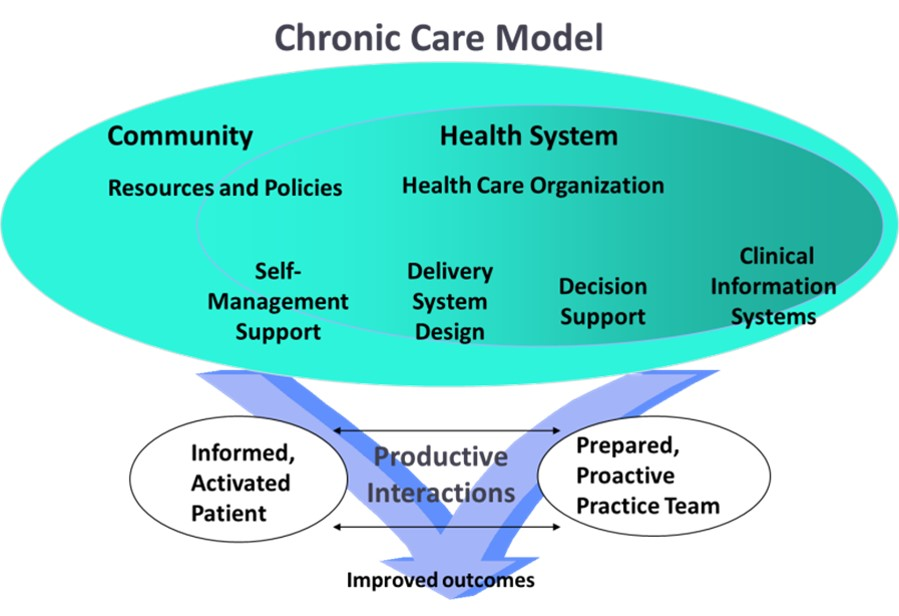
\includegraphics[width=0.8\textwidth]{chapters/2_background/chronic_model}
            \caption{Chronic Care Model}\label{fig:chronic_care}
        \end{figure}

        The same lifestyle and dietary changes mentioned in the previous section are applied by the patients during the management phase, paired with a medication plan. On a broader scale, the Chronic Care Model was designed to improve the quality of chronic disease management for primary care \cite{bodenheimer2002improving}. The model recognizes six essential elements in chronic care (figure \ref{fig:chronic_care}):
        \begin{itemize}
            \item Community resources and policies: mobilize community resources to meet the needs of patients. Education classes, self-help groups, and exercise programs are examples of such resources.
            \item Health care organization: create an organization that provides safe and high quality care. 
            \item Self-management support: patients need to be trained and given the necessary tools to effectively self-manage their chronic disease. This is an important element of telemonitoring (section \ref{2_telemonitoring}).
            \item Delivery system design: alter the structure of the medical practice to ensure effective care and self-management support.
            \item Decision support: promote care consistent with scientific data and patient preferences.
            \item Clinical information system: organize data to facilitate effective care.
        \end{itemize}

        \noindent Improvements in chronic disease management and reduced health care costs have been observed after implementing this model \cite{bodenheimer2002improving_2}. Of these elements, most studies focus on self-management support interventions \cite{reynolds2018systematic}.  Here, a key aspect is patient education as it affects the patient's perception of the effectiveness of the intervention \cite{wallace2010influence}. Self-management is heavily facilitated through telemonitoring, which the next section covers.

    \subsection{Telemonitoring} \label{2_telemonitoring}
    % between consultations
    % in relation to EHRS
    % transfers burden partly to patient
    Monitoring patients at a distance through the use of information technology is called telemonitoring \cite{systematic_review}. Here, the patient uses special monitoring devices to gather data which in turn is sent to the health care provider. While many health conditions can be monitored, telemonitoring is most prevalent in chronic disease management discussed in the previous section. A study showed that the complications of chronic diseases and costs can be reduced by the use of telemonitoring. Also, care can be provided without the use of hospital beds and the time spent managing the disease is lower \cite{telemonitoring_current_state}.

    To get a better understanding of telemonitoring and which parameters are measured, an overview of its application to chronic disease management is given. Second, the difficulties surrounding telemonitoring are mentioned.

        \subsubsection{Chronic disease management}
        A lot of studies have been conducted to test the effect of telemonitoring on chronic disease management. For all but one of the four disease categories mentioned in section \ref{chronic_diseases}, general literature was found: the literature found on cancer focussed on very specific types of the disease and not in the general sense. Consequently, only the application of telemonitoring on the other categories is discussed.

        \paragraph{Cardiovascular diseases} One study recruited 390 patients to test the effect of telemonitoring on reducing hospital days and total costs \cite{tompkins2010randomized}. 193 individuals in the intervention group were to take daily measurements using special hardware. The hardware recorded the weight, blood pressure, heart rate and blood oxygen levels. Diabetes patients received an additional blood glucose meter. Patients were also required to fill in a predetermined set of questions every week. On the clinician's end, nurses were shown a summarizing table indicating if the sent results were good, bad or missing. Based on these results, the nurses decided to contact the patient if extra care was required. The study concluded that telemonitoring appears to facilitate more efficient outpatient care and potentially reduce costs. The total numbers of hospital days for the patients in the intervention group showed a tendency to be lower and fewer emergency department visits. However, there were more urgent care and primary care visits.

        Another research paper reviewed 30 studies and noted that most patients had a positive experience and little difficulty with telemonitoring technology \cite{inglis2010structured}. In total there were more than 9500 patients in the studies. The summary concluded that there were fewer deaths, fewer hospital admissions and improved quality of life. There were also hints of reduced cost, but most studies did not report on this topic. None of the studies reported on the optimal duration of for telemonitoring.
        
        However, the effect of telemonitoring treatment on cardiovascular patients is still unclear. A paper criticized the aforementioned one, stating that the conclusions made were only valid for small studies. For large trail studies no significant effect was found \cite{chaudhry2010telemonitoring}.

        \paragraph{Diabetes} Due to the majority of research reporting on telemonitoring for diabetes type 2, literature concerning type 1 was omitted. Since diabetes is a long-term disorder, combining the management of diabetes with telemonitoring is well documented in research literature.

        One study required 32 patients to take blood glucose measurements for nine months using a Bluetooth capable glucose meter. The meter sent the measurements to a mobile phone which in turn forwarded them to a hospital server. Based on the measurements clinicians would review them and send recommendations to the patient and their general practitioner. The results showed a decrease in HbA\textsubscript{1C} from 8.40\% to 7.76\%. Higher values indicate poorer blood glucose level control. Due to the low amount of patients, the paper concluded that the benefit of telemonitoring would likely be small \cite{istepanian2009evaluation}.

        Diabetes also has an effect on blood pressure, as approximately 50 to 80\% of diabetes type 2 patients suffer from hypertension which in turn can lead to cardiovascular disease. A target blood pressure level for diabetes patients is 130/80 \cite{landsberg2004diabetes}. One study kept this goal in mind and developed a home telemonitoring program \cite{logan2012effect}. It is labeled as `home' due to the fact that a smartphone generates self-care messages for the patient, based on multiple previous readings. The results, however, would still be sent towards the clinician. Careful reviewing the data and corresponding with the patient would not be necessary thanks to the generated messages, ultimately saving the clinician time. There were 55 patients in the telemonitoring group and as well in the control group. Both groups were required to measure their blood pressure using a device, but only the telemonitoring group had the device connected to a smartphone, generating the self-care messages. The results showed that the blood pressure only decreased significantly in the telemonitoring group. Also, the percentage that reached the 130/80 target blood pressure was 51\% for the telemonitoring group and only 31\% for the control group. Last, it was suggested that the self-caring nature of the program might have negative psychological effects, requiring future study.

        Weight loss also influences blood sugar. The Active Body Control Program reported the effects of telemonitoring in combination with a dietary program \cite{luley2011weight}. The subjects were obese with diabetes type 2. A device gathered measurements from a weighing scale and an accelerometer. This device regularly sent these measurements to the hospital server. After six months significant improvements in blood sugar and weight loss were observed. No relevant changes were observed in the control group.

        Lastly, medication management is also linked to telemonitoring and diabetes. A study asked 64 patients (the telemonitoring group) to measure their blood glucose, blood pressure, and weight on a daily basis \cite{stone2009active}. A nurse would receive these measurements and adjust the medication intake five times a week. The control group consisting of 73 patients also took measurements of the same parameters, but they only received a phone call once a month to have their medication schedule adjusted. The results noted a significant decrease in HbA\textsubscript{1C} for the telemonitoring group after three and six months, compared to the control group.

        \paragraph{Chronic obstructive pulmonary disease} A 2003 study investigated the feasibility of telemonitoring for patients with COPD \cite{maiolo2003home}. In the first phase of the study 23 patients were observed for 12 months during their medical visits. For the second phase, patients were given a device which uses a finger clip to measure the oxygen saturation and heart rate. This device sends the data towards the caregivers. The caregivers analyzed the measurements and communicated comments on the symptoms and prescription changes to the patients. Results noted decreases in the numbers of hospital admissions (50\%) and acute home exacerbations (55\%). The hospitalization costs were 17\% lower compared to the first phase and 96\% of the patients were satisfied with the telemonitoring equipment. However, it should be noted that the sample size was small.

        Another study observed the quality of life of telemonitoring compared to usual care \cite{lewis2010home}. The control group received standard care for 52 weeks. The telemonitoring group received devices asking them questions about their symptoms twice a day. Also, the temperature and oxygen saturation were recorded by the device. If two of these measurements crossed a threshold, the respiratory nurses received an alert and called the patient. Between the two groups there were no significant differences seen in the quality of life, meaning that telemonitoring had no effect on this outcome.

        % data accuracy, adherence, integration EHRS, training of users...
        % technology awareness, intrusiveness, training of users
        \subsubsection{Issues}

        % inconclusive & inconsistent results
        % small sample sizes
        % many variables
        Many issues still surround the research base of telemonitoring \cite{systematic_review}. Due to the small sample sizes present in a lot of studies, results often are inconclusive or not significant. On top of that, some report positive impacts while others seem to observe the opposite. A possible cause of these inconsistencies is the fact that these studies have to deal with many variables. Characteristics such as age, technology experience, and the stage of the disease can all influence the observed results. It is important that these variables are carefully noted and considered when evaluating the results.
        
        % adherence seems high, decreases overtime in some studies
        % critical for success
        % chronic diseases need long follow-up
        The effect of telemonitoring ultimately depends on the adherence of the patient. Many studies report that the adherence of the intervention group was great, but others reported that it decreased over a long period of time. Due to chronic diseases requiring long follow-up, long-term adherence is key for telemonitoring to be successful. 

        % few reports on costs, cost benefit analysis
        %       -> economic viability -> needs longer studies
        % few reports on effect health services: ER visits, lengths of stay, hospitalizations
        Few studies report on the effects on health care costs. A couple of studies report on the daily costs of a system or program, but long-term analysis was never mentioned. This is an important factor, since telemonitoring needs to be economically viable before health care providers will adopt it. Also, the impact of telemonitoring on the utilization of health services needs to be investigated further. These services include emergency room and clinic visits, hospitalizations, and lengths of stay. 
        
        % well received and accepted
        % data accuracy, technical errors
        % still to consider
        Last, studies widely reported that telemonitoring was well received and accepted by the patients. As mentioned before, variables such as age can influence this. Also, the measuring devices reported accurate data and few technical issues occurred. However, these factors are still important to keep track of.

    \subsection{Dashboard design} \label{2_dashboards}

    Dashboards are used in many contexts. The most common examples include a car speedometer and stock analysis. In computer networking, dashboards are used to quickly interpret network traffic. In our case, we want to gather all telemonitoring data for a specific patient. To create an effective dashboard, multiple design principles should be kept in mind.
    
    While some dashboards provide fancy graphics, many miss the key point of what they are supposed to accomplish. The primary goal of a dashboard is clear communication, which is achieved through effective design. A formal definition is as follows: ``A dashboard is a visual display of the most important information need to achieve one or more objectives; consolidated and arranged on a single screen so information can be monitored at a glance.'' \cite{dashboard}. This definition contains four key characteristics:

    \paragraph{Dashboards are visual displays.} It is important that data is represented visually. Displaying charts and other graphics allows more efficient communication compared to textual information. For example, trends and outliers are easier to spot in a line chart compared to a table with the same values. Instead of using a different visualization for the sake of variety, one should always use the visualization which is best suited to effectively communicate the data \cite{few2005intelligent}.

    \paragraph{Dashboards display information needed to achieve specific objectives.} The data that is shown, must be of use for the job that needs to be done. It is possible that the data needs to be gathered from multiple sources and tailored to the specific context so an efficient visualization can be created.

    \paragraph{A dashboard fits on a single computer screen.} In order to see all information at a glance, scrolling must be prevented. If multiple screens are present, then it is no longer a single dashboard. This leads to another question: what type of display is the information shown on? Due to the wide variety of screen sizes and aspect ratios, a responsive dashboard would be most beneficial.

    \paragraph{Dashboards are used to monitor information at a glance.} Important data should be immediately noticed, whereas very specific details should be hidden. This means data must be summarized or aggregated in order to be effectively shown. However, if the user wishes to view the detailed data, the dashboard should provide means to do so.\\

    \noindent To create an effective dashboard, the user-base must be well known and understood. What type of users are we dealing with? What are their characteristics? These are important questions to ask, as one user may not comprehend one visualization while another one can. This means that the focus should be put on the user \cite{brath2004dashboard}. We can ask the following question to better understand the user's needs:
    
    \begin{itemize}
        \item What metrics does the user need to see?
        \item What context does each metric require to make it meaningful? Do we need to visualize the variance, target to reach, trend\ldots?
        \item What visualization best communicates the metric?
    \end{itemize}

    \noindent On that end, sketches and mockups can significantly help the design process. Multiple iterations, each incorporating feedback from the users, ensure that the end result is satisfactory. In section \ref{design} created paper mockups are showcased together with an explanation on the design choices.

    \subsection{Data privacy \& standards}
        
    Although out of the scope of this thesis, data privacy and the use of health standards are important components of health software. Therefore, it is important to mention them. From the onset of the design phase, data security and standard choices need to be kept in mind. When purchasing a commercial system, these aspects should also not be forgotten.

        \subsubsection{Privacy} \label{2_privacy}

        Privacy refers to the desire of a person to control the disclosure of personal health and other information \cite{biomedical_informatics}. On the other hand, confidentiality is the ability to control the release of personal health information to a care provider under the agreement that the information will not be spread or used further. Security is the protection of privacy and security, which is achieved through policies, procedures, and safeguards.

        We can ask several questions related to health information data access and storage: who owns the data? Is it the health provider or the patient? What type and how much of data needs to be stored? Who can read the data? Who can write to the data? Can someone access specific health information without consent? In order to deal with the some of the challenges concerning data access and storage, these questions need to be answered \cite{meingast2006security}.

        Striking a balance between free access to information and protection of privacy and confidentiality is difficult. Should too much information be widely available, the chance that the data is inappropriately used increases. Also, if not enough information is accessible, areas such as clinical research are hindered. Data pooling becomes less viable, preventing the analysis of disease incidence and intervention. The access to data of many patients is also important for epidemiology.

        Compared to paper records, electronic records are easily accessible, such as through the internet. This increases the chance of data breaches. Authentication, data encryption, access control, and audit logs can limit the impact of these breaches. Therefore, clear rules should be defined on who can access what data and from where.

        Through policy approaches, malicious use of health data can be prevented. Education and training programs for the medical staff will raise awareness. Also, there should be clear punishments should a privacy rule be violated. This can be tracked electronically through audits, but for paper records this is near impossible.

        \subsubsection{Standards} \label{2_standards}

        When excessive diversity creates inefficiencies and affects effectiveness standards are required \cite{biomedical_informatics}. A hospital contains many independent units spread across primary, secondary, and tertiary care. These units use software best fit for their practice and all record different data types. As such, the hospital admissions system records patient diagnosis, the pharmacy records that prescriptions were handed out, and the laboratory system records test results. Inevitably, transfer of data between the units is required. 

        To coordinate multiple systems, data transfer is essential. Nowadays too many different systems exist to create point-to-point interfaces. The creation of standards tries to resolve this. It should be noted that during the standard development creation process, instead of what is best, self-interest of the stakeholders is the main consideration. Another requirement of standards is that data can be easily stored and presented towards the users of an EHRS. Last, security measures, such as authentication and access control, need to be present.

        The use of standards in an EHRS leads to increased integration which in turn leads to lower development costs. Having to integrate many proprietary data structures will lead to complex software and a higher chance of components breaking. New medical devices and software that comply to standards prevent this.

        Health Level 7's standards are one of the most used and implemented. These messaging-based standards are created to exchange clinical and administrative data. Another standard such as DICOM is used for the communication and management of medical imaging information \cite{mildenberger2002introduction}. Medical devices interface standards are created by IEEE. Many more standards exist, but these are the more prominent ones.


	\section{Design} \label{design}

After the literature study, a design for the dashboard solution was made. What follows is a short explanation of the design process that was used. Based on the topics mentioned in section \ref{background}, a proposal was made to tackle some of the highlighted problems. Hereafter, personas and scenarios hint at the functionality and usage of this new system. Last, the components of the system, together with paper-mockups, are described.

    \subsection{MuiCSer} \label{2_muicser}
    % description of process
    This section describes the MuiCSer framework, made for user-centered software engineering processes in a multidisciplinary context \cite{muicser}, which was used to create the prototype. This framework focuses on optimizing the user experience during the entire software engineering cycle to ensure that the end-user's needs are fulfilled. By combining user-centered design and software engineering principles the user experience of the final product can be improved substantially of the final product.

        \subsubsection{Process}
        
        \begin{figure}[!t]
            \centering
            
\includegraphics[width=0.8\textwidth]{chapters/3_design/muicser}
            \caption{MuiCSer process}\label{fig:muicser}
        \end{figure}

        The MuiCSer process is summarized in figure \ref{fig:muicser}. After each phase, the result is evaluated, verified and validated to ensure that the required functionality is present. The received feedback can, in turn, be used to reiterate over the previous phase. On the figure, this is denoted with the light arrows, while the dark one represents the overall process direction.

        \paragraph{New or legacy system} At the start of the process an existing system in need of improvement is either evaluated or a new one has to be designed. This requires an analysis of the tasks and needs of the user, as well as the objects and resources required to perform these tasks. Personas and scenarios are the resulting artifacts of this phase. First, personas describe the personalities of the potential end users including hobbies, skills and the environment they surround themselves in \cite{persona_scenario}. Its goal is to uncover behavior patterns which can be of use when designing a user interface. Second, a scenario is a story describing the use of a fictitious system from the persona's point of view \cite{persona_scenario}. It tries to sketch the usage of the system for which a design must be made.

        \paragraph{Structured interaction analysis} During this phase, the results of the analysis are used to create task models. These models specify concrete tasks and goals which can be dissected into specific actions or steps the user has to take. These artifacts lay the foundation for designing a user interface which supports these tasks and goals.

        \paragraph{Low fidelity prototyping} When the actions have been specified using the task models, low fidelity prototypes can be designed. Paper sketches and mockups are such examples and are ideal for visualizing the layout of the software its user interface. Without spending too much time and resources, presenting such prototypes can yield valuable feedback from the end-user or customer. However, there is no interaction present. Typically multiple versions of these prototypes will be created until the customer is satisfied after which high fidelity prototypes can be developed.

        \paragraph{High fidelity prototyping} Creating high fidelity prototypes requires a lot more effort compared to low fidelity prototypes, as they offer functionality closely resembling the final product. However, the feedback will be much more valuable as not only design, but also functionality is tested.

        \paragraph{Final user interface} When the latest iteration of the high fidelity prototype satisfies all user requirements, the final user interface can be created. It would be beneficial to reuse the code from the prototype in order to save time and resources. As a final step, the task models are checked against the interface to check if all required functionality is present.

    \subsection{Proposal}
    
    The proposal features three core concepts which will be combined to form one cohesive solution: a dashboard, telemonitoring of chronic diseases, and customization. As mentioned in the introduction, multiple applications and integrating them pose several difficulties: data is spread and stored multiple times. Interaction between these applications is not present and integrating them requires work from the IT staff from the institution. This becomes increasingly difficult as more applications are added. To remedy this problem, a dashboard solution can gather all relevant data into one place.

    A module-based approach towards the dashboard allows easy customization and integration. Each module will serve its own purpose by showing data for one particular health parameter. As mentioned in section \ref{2_telemonitoring}, parameters such as heart rate and blood pressure are often measured to monitor multiple chronic diseases. Integration is handled by the fact that each module is independent and does not require other modules to work properly. This also helps with customization as a clinician can choose which modules are relevant for the patient in question.

    The modules that will be developed are for use in chronic disease monitoring. However, modules can be developed for purposes more fit for in-patient care. Examples are real-time monitoring, documenting diagnoses, and viewing of lab results. Which modules will be implemented and what each one of them tries to achieve is described in section \ref{design_modules}. The implementation section will provide more insight on how this independence is achieved and how future modules can be easily integrated.

    This combination allows the clinician to customize the dashboard according to each patient's needs, facilitating effective care. Data is found rapidly, albeit summarized or detailed, and not hidden away behind multiple screens. future applications should be able to create modules that will fit into the dashboard, negating the use of multiple applications. The following section describes how the system will work and how the users interact with it.

    \subsection{Personas \& scenarios}

    Based on the proposal mentioned in the previous section, personas and scenarios have been created to get a better understanding of its users and how the system will work. Each of these tries to highlight the problems the users face and how the new system tries to solve them.

        % highlights customization and dashboard
        \subsubsection{Jake}

        \paragraph{Persona} Jake is a 25-year-old male who currently works as a nurse at the hospital in his city. He has been working for 4 years for the hospital and lives alone in his apartment. Still being a young adult, Jake grew up with technology. As such he experiences no difficulties when using new software on his computer or smartphone. His hobbies include music, playing the guitar, and video gaming.

        Currently, the workflow at the hospital is dated. A new health information system was introduced to summarize and gather all medical data in a singular space. Because this is a monolithic system, a lot of features that Jake does not need still clutter the screen. Navigating the system is a pain and customization is not present. Jake wishes to only see the features he uses most while hiding the features he does not need.
        
        \paragraph{Scenario} Jake starts his first day using the new system by reading the manual that is accompanied with it. He starts the application and for each patient he is presented with a few standard layouts to choose from, based on illnesses: cardiovascular diseases, respiratory diseases, diabetes and a few others.

        After selecting a standard layout, Jake is given the opportunity to customize the dashboard. The dashboard contains all the wanted functionality of the system, where each ``block'' represents a module that can be added or deleted. Jake enters the edit mode enabling him to move the blocks around and arrange the order. He deletes a few modules and now he wants to add other modules. Jake opens the modules window where he is presented with all the available modules. A module is added to the dashboard when Jake selects it.

        By examining the new module Jake quickly notices that on the dashboard a summary is given. But when Jake clicks on the module, the block expands to fill the whole screen where detailed information is given. Jake feels he is in control of the system and that it will improve his productivity.\\

        \noindent This scenario highlights the benefits of customization. Hiding unwanted components, while adding the useful ones allow for a clear dashboard to be displayed. The user is in control and is able to quickly view data of importance. It is also possible to view detailed data.
        
        % highlights customization
        \subsubsection{Dan}

        \paragraph{Persona} Dan is a general practitioner since he graduated from university. He is on the job for 21 years and he is the preferred doctor in his town. Throughout the years Dan has used a multitude of systems and he always tries new ones to improve his workflow. Because he has been a general practitioner for such a long time, he has 500 patients that visit him at least twice a year. Some patients, especially the elderly, visit as much as once a month.

        Most of Dan's patients visit for illnesses such as fever and a cold. To diagnose these illnesses no data is necessarily needed, just a description of what the patient feels will suffice most of the time. If Dan performs such a diagnosis, he promptly adds it to the information system and to the electronic health record of the patient.

        However, if a patient visits that has a lot of problems regarding his blood pressure, then Dan has to perform a more complex diagnosis using historical data. In the current system that Dan uses, it is very difficult to search for this data. But what bugs Dan the most is that he has to do it every time this patient visits.

        \paragraph{Scenario} Because of Dan's ongoing curiosity, he tries a new health information system which allows customization for each specific patient. Because the diagnoses of most patients can be very different from time to time, Dan creates a default module group which is displayed for each patient, unless that patient has a specific module configuration. The default module group includes past diagnoses, known allergies, patient information (blood type, last weight, height\ldots) and medication list.

        The first patient of the day describes what sounds like a fever. Dan confirms this and prescribes the patient some medicine. The diagnosis is added to the `past diagnoses' module and the prescribed medication to the `medication list' module. Dan did not need other health data to perform the diagnosis. Therefore, Dan does not change the configuration of this patient.

        The next patient, an elderly woman, came for her second visit of this month. Dan knows from the past that it will probably be a heart problem. Dan searches for a `heart' module and adds it to the configuration of the elderly woman. Now both the default module group and a heart rate module are present, which is unnecessary according to Dan. He removes some modules of the default module group. Now, the next time the elderly woman visits, that configuration will be loaded.

        One specific patient had broken his arm three times in less than a year. When the patient came for a routine visit, Dan immediately added a module to easily view x-ray photos and view them in a timeline.\\

        \noindent Again, the benefits of system customization for each patient are obvious. Initially, it will take some time to configure each dashboard for all of the patients, but the system will try to provide default layouts useful for certain types of care. Once the configuration is done, the time spent during a consultation will decrease.
        
        % highlights telemonitoring
        \subsubsection{Emily}

        \paragraph{Persona} Just like Dan, Emily has been a successful general practitioner for quite some time. However, she has different needs of an EHRS. Between each patient visit, there is a period of time in which Emily does not know what happens to patients regarding certain parameters. For example, if a person has to regularly measure his heart rate and blood pressure because of cardiac disease, it is imperative that the doctor is made aware of these values. If Emily sees that these values are not looking well, she can contact the patient to come in for a checkup.

        If a patient has sleep issues, Emily wishes to not see detailed measurement values, but regular descriptions of the night’s sleep. This includes the hours of sleep, amount of wake-ups, subjective feeling of tiredness. Currently, Emily has no way of regularly receiving this information without having the patient visit, because it needs to be documented at the practice.
        
        \paragraph{Scenario} Emily recently received notice of a new platform that includes telemonitoring support. Several mobile applications are developed that can send data using an API to the platform, which in turn processes the values and can notify Emily of any anomalies. It includes customization for certain parameters in which Emily can individually assign thresholds for each patient.

        A patient who recently had a cardiac arrest is continuing rehabilitation at home. However, the patient has chest pains and pays Emily a visit. She tells the patient to regularly measure his blood pressure and heart rate, and to take note of these values in a mobile application. This application also allows taking general notes, such as feeling pain or having caught a cold. After they have scheduled the next visit, the patient is sent home.
        
        As the next few weeks pass by, Emily is notified that this patient has crossed a threshold regarding his blood pressure. Immediately Emily checks the measured data and sees a graph of all measured values. This dataset delivers insight into the history of the patient and Emily sees that there is currently no need to panic. She decides to not take action and configures a weekly reminder to keep monitoring the blood pressure.
        
        The next week, Emily receives a notification that the patient has made a note. It reads that he experienced chest pains. Again, Emily takes a look at the blood pressure data and sees a worsening trend leading to hypertension. Emily decides to call the patient to schedule an early visit. The system helped Emily to intervene as soon as the situation seemed to worsen while avoiding having the patient visit too early which in turn saves Emily time.
        
        Another patient has sleep issues. Emily encourages the patient to use a sleep monitor, which is a wristband. This device is connected to a smartphone which communicates the quantitative data to the new platform. The application on the smartphone allows the patient to take note of qualitative data such as a general description of the night or what food he/she ate. One night the patient slept only three hours and took note that he went out and drank a lot of alcohol. This could explain for example the bad sleeping rhythm for the next few days. Emily wishes to keep track of this patient on a weekly basis and configures the platform to notify her.\\

        \noindent Here, the effects of telemonitoring are highlighted. By generating reports and alerts, the caregiver can intervene when necessary. Combine this with the aforementioned dashboard platform, greater efficiency of care can be accomplished.

        % highlights integration
        \subsubsection{Anna}

        \paragraph{Persona} Anna is a software engineer working at the local hospital. From the early 2000's, she was responsible for the integration of health software systems. As such, she has experienced the continuous change associated with health software. Each unit of the hospital uses different software, while they all share a general system to view patient records. The interaction between these applications is one of Anna's responsibilities.

        As time goes on, new software and medical instruments that improve workflow are purchased. Sometimes these replace old systems, otherwise they are added to work alongside them. Both are becoming increasingly difficult to do, as the codebase of the EHRS grows. When an older system gets replaced, Anna has to weed through the code and delete little pieces, hoping other parts wont break. It is a frustrating task as often band-aid solutions are applied.

        \paragraph{Scenario} A new EHRS was installed that should improve integration of other applications. Anna skims through the documentation and starts the transition process. She quickly notices that for each device or application she needs to create a backend data structure and a module that represents it in the EHRS. The new EHRS is designed that these modules can serve as complete standalone applications or be part of a set of modules.

        After the initial transition period, everything is put into place. Not soon after, a new bedside monitors with accompanying software was purchased. These replace the old bedside monitors and consequently, the software. Thanks to the new EHRS, Anna deletes the old module without much hassle. Also, she refit the backend data structure to work with the new device's readings. This ensures that the old device data is still intact. Anna designed the new module to be similar in appearance and functionality. After implementing the module, the staff barely notices any change and workflow resumes with minor disruption.

    \subsection{Modules} \label{design_modules}
    
    As mentioned in the proposal, the dashboard will feature a module-based design. This section will describe the modules that will be built in the prototype. For each module, the reasons behind the design choices are given, as well as a low-fidelity paper mockup. Keep in mind that all modules are primarily chosen to aid with chronic disease management.

    Each module has its own design, which is in line with the principles mentioned in section \ref{2_dashboards}. For each module we ask the following questions:
    \begin{itemize}
        \item What functionality does the module offer?
        \item What data will it represent?
        \item How do we show as much data as possible at a glance?
        \item How are summaries generated?
        \item How are the detailed values shown?
    \end{itemize}

    Some functionality is present in all modules. These include resizing the module to a larger or smaller version with varying amounts of detail, increasing the customization options. The smaller the module, the more data is aggregated to a summary. Each module can be freely placed anywhere on the dashboard. Also, all modules can navigate through historical data either by week or by month. The ability to set thresholds for each patient is always present, which is necessary to generate appropriate alerts.

    Based on the telemonitoring literature review from section \ref{2_telemonitoring}, the following modules will be created:
    \begin{itemize}
        \item Heart rate: cardiovascular disease, diabetes, and COPD.
        \item Blood pressure: cardiovascular disease and diabetes.
        \item Blood sugar: diabetes.
        \item Weight: cardiovascular disease and diabetes.
        \item Oxygen saturation: cardiovascular disease and COPD.
        \item Medication: cardiovascular disease and diabetes.
    \end{itemize}

    % dashboard
    \subsection{Other components}



	% chktex-file 36

\section{Implementation}\label{implementation}

This section describes the implementation process. The design highlighted the usage of the dashboard through its personas and scenarios, while the low fidelity mockups gave an early glance at its appearance. At its core, the strength of the application revolves around its extensibility and usability. Therefore, a lot of thought went into choosing the best libraries to provide these features.

First, an overview of the entire application is given, after which we go into more detail. The dashboard consists of two major parts common to web development. The back end is described first. This section explains the reasoning behind the chosen technology stack and the general structure. We also specify the back end structures and REST API calls for each module and component which the front end has access to. For the front end, we explain how the Polymer 3 library supports our modular design and its underlying principles. Hereafter, other libraries used during the implementation, the general front end structure, and the resulting dashboard and its modules are explained. 

It is without question that during the implementation small changes were made to the design. These changes are documented for both parts. During the entire development process, only basic authentication was implemented. The implementation of standards, privacy rules, and security techniques do not contribute towards the goal of the dashboard we defined in the design section. Therefore, we consider these topics out of the scope of the prototype.

    \subsection{Overview}

    The first major choice that was made, was the type of application to develop: a native application or a web application. It was a relative simple choice, but nonetheless an important one. Native applications are developed, in most cases, for one type of operating system. If a vendor wants to support both Android and iOS devices, two separate applications need to be developed. This requires more developers to not only create the application, but also to maintain it. Another drawback of native applications is the update process. This process often requires the reinstallation of the entire application, which is very disruptive and difficult to do in a care setting.

    Web applications saw a surge in popularity. Compared to their native counterparts, web applications today are becoming increasingly similar in terms of functionality and design. Office Online from Microsoft is a good example showcasing this, which features many functions found on the desktop versions of the Office Suite. While these web applications also require updates, these happen on the server side. When the user refreshes the web page, the latest version of the application is automatically retrieved. This simplifies the roll-out process significantly. Also, all operating systems that support web browsers, are capable of running this type of applications. This includes mobile devices. As a result, developers only have to develop one application. However, the variation in screen resolutions and aspect ratios calls for a responsive design.

    With this in mind, the choice to create a web application was evident. Users can view the dashboard regardless of the device they use, without sacrificing functionality. It should be noted that complex operations will not fit easily into a web application. The strength of web apps also leads to its major drawback: poor performance. A native application can draw much more computational power from the device it was made for. To transfer the computation burden to the server is also not a viable solution as this puts additional strain on the network. In case of real-time applications, latency becomes an issue due to continuous data transfer. However, the dashboard application should not experience any performance issues as the modules that were defined in section~\ref{app_specification} do not require complex operations.

    \begin{figure}[!t]
        \centering
        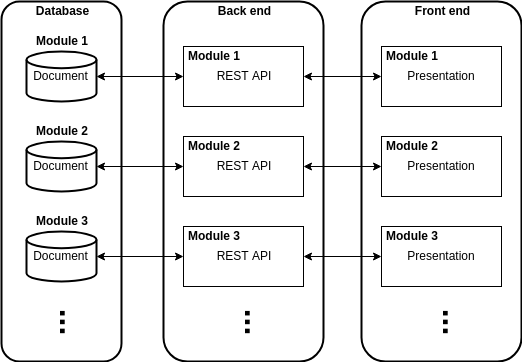
\includegraphics[width=1\textwidth]{chapters/4_implementation/structure}
        \caption{The communication flow by which every module communicates.}\label{fig:structure}
    \end{figure}

    A typical web application consists of two parts: the back end and the front end. In software engineering principles, these refer to the separation of the data access layer and the presentation layer of the web application. For example, the back end fetches data requested by the front end. In turn, the front end presents the retrieved data towards the user. Due to the modular design of the dashboard, each module needs to have its own back and front end structures, visualized by figure~\ref{fig:structure}. As the figure indicates, there is no direct interaction between the modules, which facilitates low coupling. The next sections describe the back end and front end in detail. Changes made to the design from section~\ref{design} are explained whenever they occur.

    \subsection{Back end}

    \begin{figure}[!t]
        \centering
        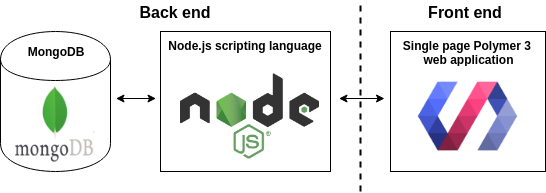
\includegraphics[width=1\textwidth]{chapters/4_implementation/tech}
        \caption{The three core technologies used to build the application.}\label{fig:tech}
    \end{figure}

    The back end is responsible for everything related to the management of the data present in the dashboard application. It is here that the logic is defined to add, update, or remove records from the database based on the requests it received from the front end. The back end exposes a REST API which determines which requests the front end can send.

    This section gives a detailed description of how the back end part of the dashboard was implemented. First, we go over the chosen technology stack after which we explain the back end structure. To close, each component present in the back end is briefly described.

        \subsubsection{Technology stack}

        Figure~\ref{fig:tech} shows the three core technologies used to develop the application. The back end was built using Node.js and MongoDB\@. We now give a brief explanation of what each back end component tries to achieve and why it was chosen.

            \subsubsubsection{Node.js}

            The back end server forms the heart of the dashboard application and Node.js was the preferred choice to implement it. Node.js (or simply Node) is a Java-Script runtime built on Google Chrome's V8 JavaScript engine~\cite{NodeJS}. Node avoids the classic thread-based approach to concurrency, which is relatively inefficient and can be very difficult to use. Instead, it provides concurrency via a single event loop that can support thousands of simultaneous connections, using non-blocking I/O calls. Node also has the added bonus of streamlining web development to the use of a single language.
            
            The main reason Node was chosen, was due to the very large collection of packages that is available through the Node Package Manager (npm). For example, the Express package is only available via Node. This package was of significant help during the entire development process. Also, documentation is easily found thanks to the very large community that develops with Node.

            \subsubsubsection{MongoDB} 
            
            A SQL database is table-based, whereas MongoDB is document-based~\cite{MongoDB}. This type of structure enables highly flexible data schemas, as new data fields can be added without affecting existing documents. This is especially useful when a new data structure from a 3rd party vendor needs to be added to the database. This supports the dashboard's goal of simple extensibility. Also, the developers of MongoDB officially support Node.

            \subsubsubsection{Node packages}

            Node allows developers to easily install a broad selection of packages. We now discuss the packages that were used for the development of the back end. These served many purposes, such as routing, encryption, logging, and request body parsing. 

            \paragraph{Mongoose} Using Node without a library to communicate with MongoDB is very difficult, as data validation and casting must be written manually. By installing Mongoose, a MongoDB object modeling package, this will be taken care of~\cite{Mongoose}. Via this package we can define data schemas and its parameters. Hereafter, a data model is created by compiling the schema. It is now possible to create MongoDB documents in a very similar fashion to object-oriented programming, which encapsulates the more complex inner workings of MongoDB\@. The entire database is constructed via these models.

            \paragraph{Express} Express is a Node web application framework, which helps with the management of routing, connecting middleware, handling requests, and others~\cite{Express}. It can also be of help with organizing a web application on the server side into a MVC architecture. Furthermore, Express makes the creation of a REST API server a much faster process compared to vanilla Node. Since we need to transfer data from MongoDB to our front end via a REST API, this framework is essential. Section~\ref{backend_structure} goes into detail how Express helped define the structure of the back end of the dashboard application.

            \paragraph{Bcrypt \& JSON Web Tokens} Basic encryption is provided by the bcrypt package~\cite{Bcrypt}. Whenever a user registers, the password is hashed and then stored into MongoDB via Mongoose. In case the user successfully authenticates, the JSON Web Tokens package generates a token based on the login name, user id, clearance level, and a secret phrase~\cite{JWT}. This token is sent back to the front end and from now on, must be embed into every future request. After one hour, the token expires and the user must authenticate again.

            \paragraph{Other} The body-parser package helps as its name implies with parsing request bodies. This package is connected to Express as middleware, since it captures the request and parses it before it lands into the developer's hands. For example, accessing parameters in the body of a POST request is done with this simple statement: \texttt{request.body.paramName}. Morgan is another helpful package which logs all requests made to the server. As such, it is a helpful debugging tool. Last, but certainly not least, is the nodemon package. Nodemon detects changes in a Node project. If changes are found, nodemon automatically restarts the server to apply these changes.


        \subsubsection{Structure}\label{backend_structure}
        
        As mentioned before, the Express framework can help with organizing a web application into a MVC architecture. As such, the entire dashboard prototype is built around this architecture. A MVC architecture consists of three parts:
        \begin{itemize}
            \item Model: the part that manages the data and receives input from the controller. This is handled by Mongoose.
            \item View: the view presents the model or in other words, the data. The front end is our view, which is a Polymer 3 server.
            \item Controller: the controller handles incoming requests from the view. Hereafter it calls the model to receive the desired data, which it then returns to the view. This is realized on the back end Node server with the help of Express.
        \end{itemize}

        \noindent Every module present in the back end has three files of the same name that are spread across the following three folders: controller, models, and routes. The following example explains how they are connected:
        \begin{myenumerate}
            \item The front end sends a request to a certain route. Express checks this route and sees that the file \texttt{routes/patient.js} uses it. 
            \item \texttt{routes/patient.js} has every possible API endpoint mapped to a controller function which executes certain logic to retrieve data. All these controller functions are found in the \texttt{controller/patient.js} file.
            \item Last, certain logic gets executed depending on which controller function is called. The controller calls the Mongoose model to perform certain actions on the database, which is defined in \texttt{models/patient.js}.
            \item Depending on the operation, the controller can send data retrieved from the model back to the view. This transaction does not pass by the router.
        \end{myenumerate}

        \noindent In order to extend the dashboard application, these three files need to be created for each component.

        \paragraph{Routing} The routes defined in the back end follow a simple structure. The application starts at the root endpoint: \texttt{/}. Suppose the server receives a request destined for the following endpoint: \texttt{/clinician/login}. At the root level, in \texttt{app.js}, the server forwards all routes starting with ``clinician'' to the routes defined in \texttt{routes/clinician.js}, due to the following line:\\
        \centerline{\texttt{app.use(`/clinician', clinicianRoutes);}}\\ % chktex 36
        All routes defined in \texttt{routes/clinician.js} are therefore called sub-routes, since they aren't defined at the root level.\medskip

        \noindent The same counts for data associated with patients, but one step further. Suppose the server gets the following request: \texttt{/patient/id123/allergy}. The server will forward the \texttt{/id123/allergy} part to \texttt{routes/patient.js}. The patient module will now forward this route to \texttt{/routes/modules/allergy.js}, due to this statement:\\
        \centerline{\texttt{router.use(`/:pId/allergy', allergyRoutes);}} % chktex 36
        
        \subsubsection{Components and dashboard modules}

        We now briefly describe the purpose of every component within the back end of the prototype.

            \paragraph{Clinician} This component allows users to sign up an log in to the system. The controller uses the previously mentioned bcrypt package to provide encryption. Also, the JSON Web Token package is used to return a authentication token should the authentication be successful. The model simply saves the username, encrypted password, and a clearance level. The last field was added to provide basic access control. However, this is not present in the prototype.

            \paragraph{Layout} The layout component allows the front end to save the current configuration of a dashboard. The model stores the patient id, user id, size of the patient info module, a list of the small modules with their corresponding heights and locations, and a list of the main modules with their corresponding dimensions and locations. The existing layout is always deleted first before the new one is saved. This ensures that only one layout configuration exists for every user-patient combination.

            \paragraph{Import} This module makes it possible to import a large set of patient data in a JSON format, which can be useful when migrating to this system. The component calls import functions from the patient component, which is described below. The data needs to be conform to the specification mentioned in appendix~\ref{json_import}.

            \paragraph{Patient} The demographic data of a single patient or of all patients can be requested via this module. The router also receives requests that are meant for the dashboard modules, as explained in section~\ref{backend_structure} during the routing example. The controller also delegates parts of its import process to the relevant modules. For example, if the import information contains a key ``prescriptions'', then the patient controller passes this data on to the prescription controller.

            \paragraph{Dashboard modules} The components related to the dashboard modules are straightforward in terms of functionality. These modules support the CRUD operations. However, the history module only allows the reading of data, since this is sensitive data that should never be deleted. Also, the history controller is called in the other controllers in order to log data changes. Additionally, the telemonitoring has sub-components for each parameter it supports. These are: blood pressure, blood sugar, heart rate, blood oxygen, and weight.

    \subsection{Front end}

    The front end serves as the face of the dashboard application and is more complex than its back end counterpart. Throughout the lengthy implementation phase several changes were made, which required some work to be redone, but in the end promotes better extensibility and usability. 
    
    A modular dashboard was built using the Polymer 3 framework in combination with several libraries. The topics web components and shadow DOM are very important in realizing loosely coupled and highly cohesive modules, which is why it is important to understand them. After the used libraries are explained, the structure of the front end is described. To conclude, the end result is shown via various screenshots of the dashboard and its modules.

        \subsubsection{Polymer 3}

        Polymer is an open-source library that provides a set of feature for creating web components~\cite{Polymer}. The library is developed by Google and contributors. Several Google services such as YouTube and Google Earth were developed with Polymer.

        HTML provides us with standard elements such as \texttt{h1} and \texttt{img}. Web components allow the developer to create custom elements which are used in the same manner as the ones HTML provides. Suppose a calendar web component was created, a developer could add the element to any web page as follows: \texttt{<calendar></calendar>}. The actual definition of the calendar module resides in another file which is imported on the page where it will be used. This approach promotes the creation of reusable components. This also means that the dashboard application can be easily extended with these components. This is largely made possible by the shadow DOM\@.

        \paragraph{Shadow DOM} The Document Object Model describes a tree of documents. The web browser builds such a tree for every web page it loads. The shadow DOM can be seen as a scoped subtree inside a custom element. The root of this subtree is called the shadow root. The structure, styling, and behavior of the children within the shadow DOM do not affect any elements outside of it. Therefore, the appearance and functionality of the custom element is encapsulated and hidden at the document level. Only events fired by elements in the shadow DOM can be caught outside the shadow DOM boundary. This idea of encapsulation is important for our approach towards the dashboard, as each module is responsible for its own appearance and functionality. Developers of custom modules should not need to worry about what happens outside of the shadow DOM\@.

        \subsubsection{Libraries}

        The dashboard must support resizing, and dragging and dropping of modules. To realize this, several libraries were compared with each other and the best fits were chosen. During this section the libraries used to create the front end functionality are described.

            \paragraph{Packery \& Draggabilly} Packery is a JavaScript library that makes gapless and draggable layouts~\cite{Packery}. As items are added and removed from the grid, Packery reorders the layout. The documentation of the library mentions that drag and dropping is supported via the Draggabilly library. This built-in support was the main reason Packery was chosen. There are two Packery grids in the prototype, one for the left panel and one for the main panel. 

            \paragraph{Interact.js} This library implements JavaScript drag and drop, resizing, and multi-touch gestures for modern browsers~\cite{Interact}. However, Draggabilly already provides drag and drop functionality. Since Interact is not supported by Packery, we can't replace Draggabilly with it. Therefore, Interact serves as the library that implements the resizing functionality for the modules.

            \paragraph{Other} The handling of dates throughout the dashboard is done via the Moment library. This library provides very intuitive manipulation methods which are of great help when communicating dates back and forth to the back end. The charts of the telemonitoring are generated via the C3 library, which is a wrapper on top of the D3 library.

        \subsubsection{Structure}

        To start, the entire dashboard is packaged as web component. The application is loaded by placing \texttt{<main-element></main-element>} as the single child in the of the body found in the \texttt{index.html} file. This opens up the ability of having multiple instances of the application open side by side. However, this was not explored further.

        All modules are placed in the \texttt{src} folder. This includes the \texttt{main-element}, but also the following web components: all modules that can be placed on the dashboard, the patient list (\texttt{patient-list-element}), and the patient information module (\texttt{patient-element}). Inside the \texttt{src/modules} folder each module is placed into its own folder. In case the module has both a small and a normal version, two files are found within this directory. Small variants of modules always end with the \texttt{-small} suffix. For example, the allergy module folder contains the files \texttt{allergy-element.js} and \texttt{allergy-element-small.js}.

        The root of the \texttt{src/modules} folder contains the following two files: \texttt{base-
        element.js} and \texttt{base-element-small.js}. These are base web components which all other modules have to extend. This gives each module a streamlined look and design. Also, these base components provide templates which may or must be overridden for the module to work with the dashboard. We describe both base components now in detail.

            \subsubsubsection{Base components}\label{base_components}

            Both base components provide the functions, interface elements, styling, and properties that all modules in the dashboard should have. They serve as a starting point for the developer when creating a new module. It saves the developer time as a basic layout along with utility functions are already defined. They also prevent code duplication. For example, the format of dates displayed in the modules is defined in the base component. Change this format in the base component and it will reflect to all other modules. The next paragraphs go into detail what both the normal and small base components provide.

            \paragraph{Normal base component} The component provides a small block in which a header is defined. This header contains a placeholder title and dialog button. A button in the top right corner to remove the module is also present in the header, which can not be overridden or removed. Five templates exist which can be overridden: 
            \vspace{-6pt}
            \begin{myenumerate}
                \item \texttt{cssTemplate}: define the CSS styling here. Is empty in the base module.
                \item \texttt{ironAjaxTemplate}: define ajax calls here using the \texttt{iron-ajax} web component. Is empty in the base module.
                \item \texttt{dialogTemplate}: define dialogs that may be opened by the module in this template. Is empty in the base module.
                \item \texttt{contentTemplate}: contains the actual content of the module. Contains a placeholder in the base module.
                \item \texttt{dialogButtonTemplate}: specify the action to occur when this button is clicked, such as opening a settings dialog to configure the module. Contains a placeholder in the base module.
            \end{myenumerate}

            \noindent The title can be overridden by modifying the property in the extending module, which the following statement does: \texttt{this.title = `Vaccinations';}\medskip

            \noindent Finally, the base component provides several functions, some of which are placeholders that need to be overridden. These functions serve either as utilities for use within the module, such as getting a formatted date string, or as a function that is called from the \texttt{main-element}, such as getting the minimum size of the module. We now list these functions:
            \vspace{-6pt}
            \begin{myitemize}
                \item \texttt{setDateFormats(datePicker)}: sets the format of the date picker if one is present in the module.
                \item \texttt{getDateString(date)}: converts a date to a string in the DD/MM/YYYY format.
                \item \texttt{getTimeString(date)}: gets the specific time from a date in the HH:mm format.
                \item \texttt{setPatientId()}: stores the id of the current loaded patient to a class variable.
                \item \texttt{update(e)}: called by the \texttt{main-element} to signal that the module should refresh its data. Needs to be overridden to send the data requests to the correct route.
                \item \texttt{sendUpdateSignal()}: should be overridden to fire a signal telling the \texttt{main-element} all instances of this module should refresh their data. The dashboard will do this by calling \texttt{update(e)} from those modules.
                \item \texttt{getMinSizes()}: called by the \texttt{main-element} when creating the module. Should be overridden by returning the minimum width and height of the module.
                \item \texttt{getSettings()}: called by the \texttt{main-element} when saving the module layout. Should be overridden to return the state of the module in case it needs to be saved.
                \item \texttt{loadSettings(settings)}: called by the \texttt{main-element} when loading the layout. Should be overridden in order to restore the state of the module.
            \end{myitemize}

            \paragraph{Small base component} The smaller component is similar to its normal counterpart. However, it is smaller in terms of what it provides. This module also contains a header with a placeholder title. The only other part of this header is the remove button. All templates except the \texttt{dialogButtonTemplate} from the normal base component are present and have the same purpose in the smaller version. The title of this module is also overridden in the same manner as the normal base component. The smaller module provides a subset of the functions of its counterpart:
            \vspace{-6pt}
            \begin{myitemize}
                \item \texttt{getDateString(date)}: converts a date to a string in the DD/MM/YYYY format.
                \item \texttt{setPatientId()}: stores the id of the current loaded patient to a class variable.
                \item \texttt{update(e)}: called by the \texttt{main-element} to signal that the module should refresh its data. Needs to be overridden to send the data requests to the correct route.
                \item \texttt{sendUpdateSignal()}: should be overridden to fire a signal telling the \texttt{main-element} all instances of this module should update their data. The dashboard will do this by calling \texttt{update(e)} from those modules.
                \item \texttt{getMinHeight()}: called by the \texttt{main-element} when creating the module. Should be overridden by returning the minimum height of the module.
                \item \texttt{getSettings()}: called by the \texttt{main-element} when saving the module layout. Should be overridden to return the state of the module in case it needs to be saved.
                \item \texttt{loadSettings(settings)}: called by the \texttt{main-element} when loading the layout. Should be overridden in order to restore the state of the module.
            \end{myitemize}

        \subsubsection{Dashboard}

        Once the user opens the application, Packery will initialize the grids found in the two panels of the dashboard. Hereafter, the user must authenticate by providing his/her credentials. If the authentication succeeded, then the patient list will present itself. If the authentication failed, the user will have to try again. Once a patient is selected, the process of loading the layout starts, which we describe in the next section.

            \subsubsubsection{Layouting}

            \paragraph{Load configuration} As soon as a patient is selected, Packery removes all modules that are present in the two grids. Hereafter, the patient information module is added to the left panel. Now the module configuration can be loaded, which consists of the following steps:
            \vspace{-6pt}
            \begin{myenumerate}
                \item Call the API to receive the layout configuration of the current patient.
                \item Load the small modules:
                \begin{myenumerate}
                    \item Create the module.
                    \item Set the configured height of the module.
                    \item Add the module to the grid of the left panel and tell Packery to place it at the location where it originally was.
                    \item Restore the state of the module by loading its settings.
                \end{myenumerate}
                \item Load the other modules:
                \begin{myenumerate}
                    \item Create the module.
                    \item Set the configured width and height of the module.
                    \item Add the module to the grid of the main panel and tell Packery to place it at the location where it originally was.
                    \item Restore the state of the module by loading its settings.
                \end{myenumerate}
            \end{myenumerate}
            
            \noindent This process only occurs when switching between patients. If there is no configuration, the dashboard will be empty.

            \paragraph{Save configuration} Whenever the user makes changes to the layout of the dashboard, the layout is automatically saved. The auto-save happens after one of the following events occur in either panel: adding or removing a module, moving a module, resizing a module, or changing the state of a module. The save process is as follows:
            \vspace{-6pt}
            \begin{myenumerate}
                \item Retrieve all main modules from Packery and retrieve their settings, and calculate their sizes and locations.
                \item Retrieve all small modules from Packery and retrieve their settings, and calculate their heights and locations.
                \item Retrieve the current size of the patient information module.
                \item Send all this information via the REST API to the back end.
            \end{myenumerate}

            \subsubsubsection{Adding modules} % en drag en drop

            The creation of the modules in itself was not difficult to do. However, an issue arose in an attempt to make these modules draggable. In order to make something draggable with Draggabilly, the library needs to have an identifier of an object such as a class name, that will serve as a drag handle. The original plan was to provide drag and drop by selecting the module title in the header of the module. This would serve as the drag handle. However, Draggabilly could not find the identifier, because it was encapsulated in the shadow DOM of the module.

            The solution to this problem was to place the web component into a container which contains a thin bar at the top that serves as the drag handle. This is automatically done for all modules and does not require extra attention from the developers. Screenshots show the small grey bar at the top of the module. The following steps were taken to create the container:
            \vspace{-6pt}
            \begin{myenumerate}
                \item Create the module and the container.
                \item Set the resize event listeners on the container.
                \item Set the minimum dimensions of the container.
                \item Create the handle with its corresponding class name.
                \item Append the handler to the container.
                \item Append the new module to the container.
                \item Set the remove and broadcast event listeners.
                \item Add the container to the Packery grid.
                \item Create a Draggabilly object for the container and bind it to Packery.
            \end{myenumerate}

            \subsubsubsection{Resizing}

            As mentioned before, the Interact library was used to implement resizable components. For small modules, resizing is only possible by dragging the bottom edge. The normal modules can be resized by dragging the bottom and right edges. In order to provide a clean layout, the modules are resized in chunks of 20 pixels. This simplifies the process of arranging into a neat layout. This was done by subtracting the remainder of the division by 20 of both the width and height during the resize. In case the new width or height is different from the current one, then the resize occurs. While resizing, Packery wil move other modules out of the way. Interact also provides a listener to detect when the resizing has ended. After each resize end, the dashboard saves the layout changes.

        \subsubsection{Modules}

        \begin{figure}[t]
            \centering
            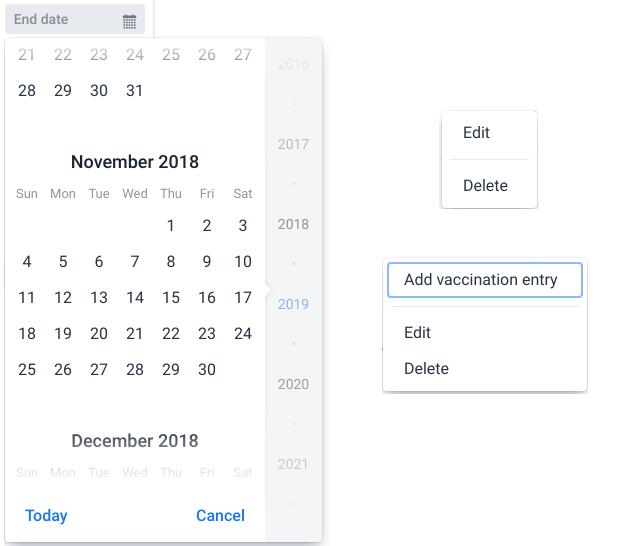
\includegraphics[width=0.8\textwidth]{chapters/4_implementation/vaadin-comps}
            \caption{Left: the \texttt{vaadin-date-picker} component, right: two examples of the \texttt{vaadin-context-menu} component.}\label{fig:vaadin-comps}
        \end{figure}

        This section provides implementation details for each module. Some 3rd party web components were used to provide features needed by several modules. These are the following: \texttt{vaadin-grid}, \texttt{vaadin-date-picker}, and \texttt{vaadin-context-
        menu}~\cite{Vaadin}. We briefly explain what role each Vaadin component has within the dashboard after which we describe the dashboard modules.

        \paragraph{Vaadin grid} The \texttt{vaadin-grid} component creates data tables that have a clear interface and has support to show details of data rows. Throughout the dashboard, all data lists are made with this component.

        \paragraph{Vaadin date picker} This component provides a date selection field. All dates are entered via this component. The user enters dates by either typing them in a correct format, or by selecting the date using the widget, which figure~\ref{fig:vaadin-comps} shows shows on the left.

        \paragraph{Vaadin context menu} The user can press the right mouse button on certain data to delete or update it. Otherwise, buttons would need to be displayed to provide these actions, which may clutter the screen. The data displayed in the Vaadin grid components can be edited this way. Two examples of such context menus are displayed on the right side of figure~\ref{fig:vaadin-comps}.

            \subsubsubsection{Patient list}

            \begin{figure}[t]
                \centering
                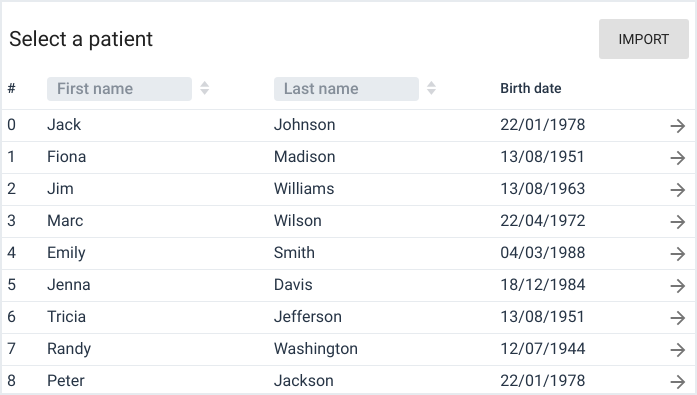
\includegraphics[width=1\textwidth]{chapters/4_implementation/patient-list}
                \caption{The patient list component.}\label{fig:patient-list}
            \end{figure}

            After successful authentication, the user sees the patient list. This list shows basic information concerning the patients that are in the system. Also, it is possible to sort and search by first or last name. As figure~\ref{fig:patient-list} shows, the user can import patients by pressing the button in the top right corner. This opens a dialog box that accepts raw JSON data. The JSON data must follow the specification from appendix~\ref{json_import}. Also, this module does not extend the base component mentioned in section~\ref{base_components} because it will never be placed on the dashboard.

            \subsubsubsection{Patient information}\label{mod_patient_info}

            \begin{figure}[t]
                \centering
                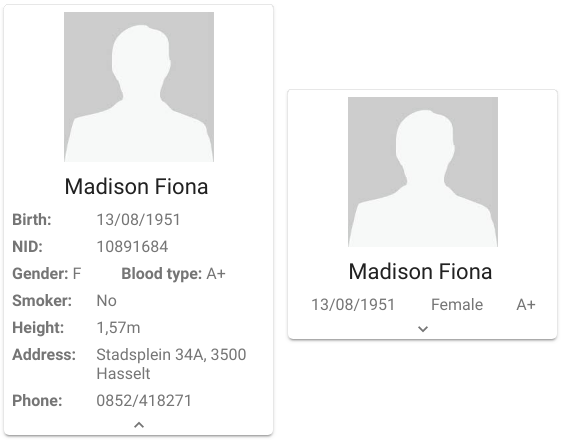
\includegraphics[width=0.8\textwidth]{chapters/4_implementation/patient-info}
                \caption{The two possible sizes of the patient information module.}\label{fig:patient-info}
            \end{figure}

            The patient information module is always present on the left panel of the dashboard and it can not be removed. The reasoning behind this, is that clinicians should always be able to see which dashboard is open. It is possible that the name of the patient only appears in this particular module and if it is removed, confusion may arise. By pressing the arrow button on the bottom, the size of the module changes, which in turn triggers a layout save. Figure~\ref{fig:patient-info} shows the two possible sizes. This was implemented by swapping between two \texttt{div}'s every time the arrow button was pressed. There are no notable changes made to this module, compared to the design. The picture at the top of the module is a placeholder. This module also does not extend the base component, because it can't be freely placed on the dashboard.

            \subsubsubsection{Prescription}\label{mod_prescription}

            \begin{figure}[t]
                \centering
                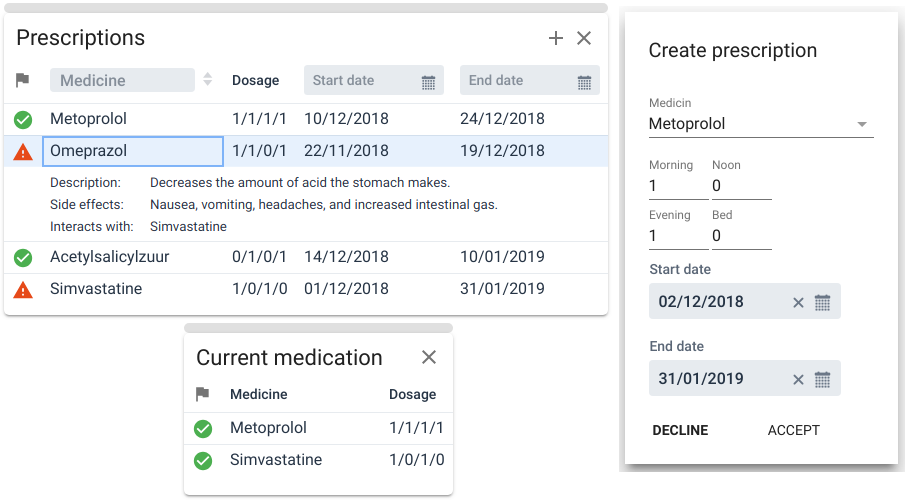
\includegraphics[width=1\textwidth]{chapters/4_implementation/prescriptions}
                \caption{The normal and small version of the prescription module. Adding prescriptions is done via the dialog on the right.}\label{fig:prescriptions}
            \end{figure}

            The prescription module is unchanged compared to the design. This module uses the Vaadin grid for both the small and normal versions to display the prescriptions, as figure~\ref{fig:prescriptions} shows. Removing and editing the prescriptions is done via the Vaadin context menu. Also, note the gray drag handle on top of the modules. In case there are interactions, the icon in the leftmost column changes. Hovering over this icon indicates the interacting medicine.

            When no dates are selected, all prescriptions that were ever assigned to the patient are shown. As soon as two dates are selected, the module checks if they are valid. These checks include that the start date must be before the end date. Every time the module receives prescriptions, it checks for prescriptions against interactions. Because this is a prototype, fictive interactions were created.

            The small module always shows the medication the patient takes of today. This gives the user a way to quickly see the current medication scheme of the patient, without showing too much details. As such, from the small module no prescriptions may be added, edited, or removed.

            \subsubsubsection{Allergy}\label{mod_allergy}

            \begin{figure}[t]
                \centering
                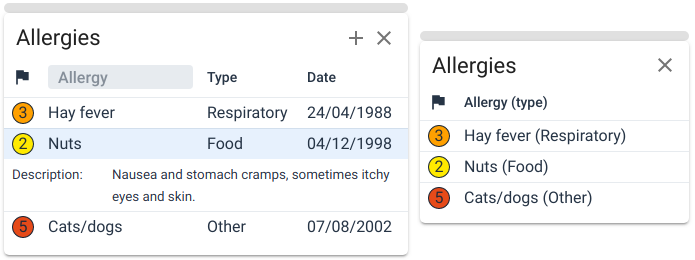
\includegraphics[width=1\textwidth]{chapters/4_implementation/allergies}
                \caption{The normal and small version of the allergy module.}\label{fig:allergies}
            \end{figure}

            The allergy module may be the simplest one in terms of design and functionality, but it still is an important part of an EHR\@. No changes were made to the design of the module. Shown in figure~\ref{fig:allergies}, a more severe reaction to the allergy is indicated by a red icon. Again, the small module only serves as a reference and no changes to the allergies can be made from here.

            \subsubsubsection{Vaccination}\label{mod_vaccination}

            \begin{figure}[t]
                \centering
                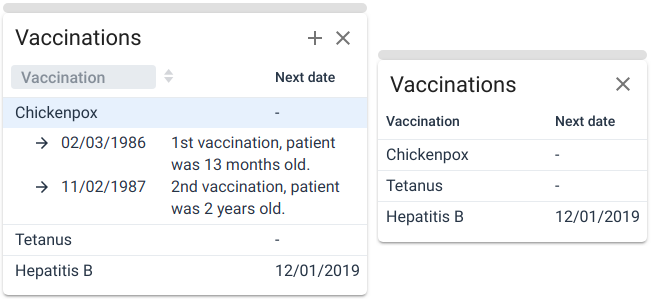
\includegraphics[width=1\textwidth]{chapters/4_implementation/vaccinations}
                \caption{The normal and small version of the vaccination module.}\label{fig:vaccinations}
            \end{figure}

            This module is very similar to the allergy module. It shows a list of conditions for which the patient is vaccinated. In case a revaccination is scheduled, this date is also shown. For each condition, historical vaccinations can be added via the context menu (figure~\ref{fig:vaadin-comps}, right). These vaccination entries have a description and a date, as shown in figure~\ref{fig:vaccinations}.

            \subsubsubsection{Workflow}\label{mod_workflow}

            \begin{figure}[t]
                \centering
                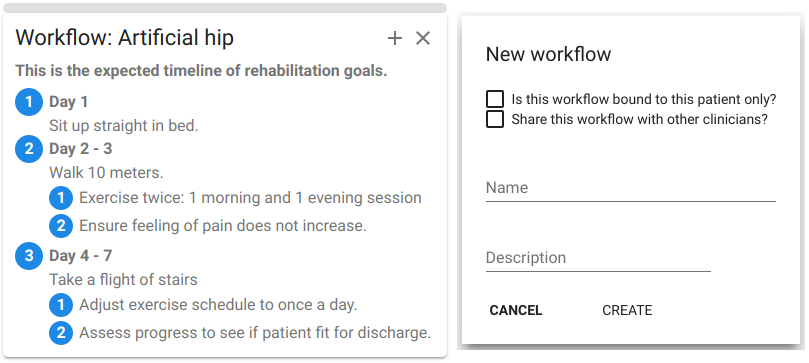
\includegraphics[width=1\textwidth]{chapters/4_implementation/workflow}
                \caption{The workflow module on the left, showing a workflow for the example mentioned in section~\ref{app_specification_modules}. The dialog on the right is used to create a new workflow.}\label{fig:workflow}
            \end{figure}

            The workflow module was difficult to implement. However, there are no significant changes compared to the design. Figure~\ref{fig:workflow} shows a workflow and also the dialog to create a new one. Whenever the user loads a workflow the layout is saved. The module overrides the \texttt{loadSettings(settings)} and \texttt{getSettings()} functions of the base component to save and load the identifier of the currently loaded workflow. It should be noted that multiple instances of this module may be added to the dashboard, with each showing a different procedure. They will not interfere with each other. Because these workflows can contain a lot of information, no small module was made. Providing a summary in this case is not useful, nor clarifying.

            \subsubsubsection{Checklist}\label{mod_checklist}

            \begin{figure}[t]
                \centering
                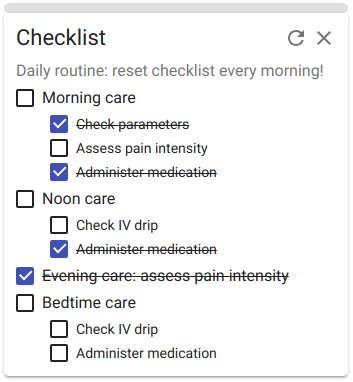
\includegraphics[width=0.5\textwidth]{chapters/4_implementation/checklist}
                \caption{The checklist module.}\label{fig:checklist}
            \end{figure}

            As a result of the workflow module, a new module not mentioned in the design was made. A checklist module was created which allows the user to add tasks and potential sub-tasks. This checklist is bound to the patient, so if one user checks off a task, it will also be checked for another user. The module was implemented by editing a copy of the workflow module, due to being similar in structure. The result is shown in figure~\ref{fig:checklist}. The button to the left of the remove button resets the entire checklist. A small module was not created for the same reasons one wasn't created for the workflow module.

            \subsubsubsection{History}

            \begin{figure}[t]
                \centering
                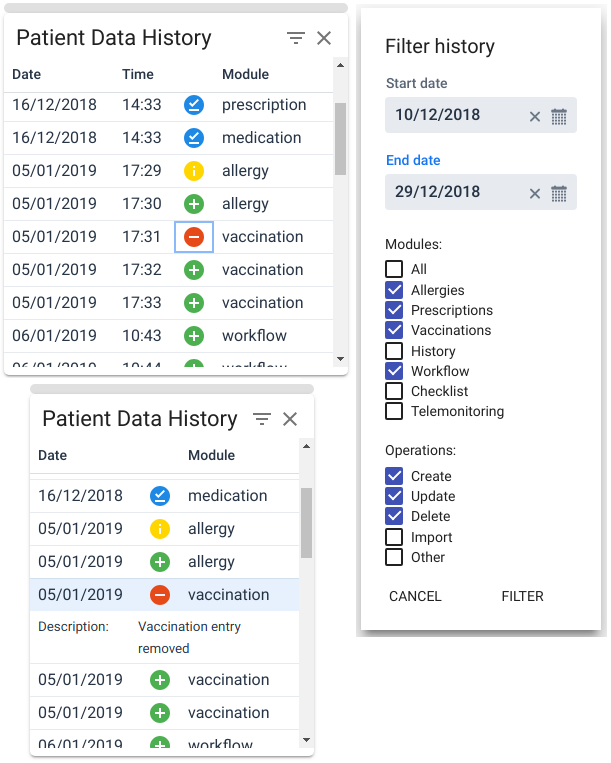
\includegraphics[width=0.8\textwidth]{chapters/4_implementation/history}
                \caption{The history module where the wide module shows an extra column. Filters are set via the dialog on the right.}\label{fig:history}
            \end{figure}

            The history module was added late in development. No significant changes were made to the design. As figure~\ref{fig:history} shows, the wider history module has an extra time column. This was an experiment regarding the resizing functionality to show and hide elements as the component grows or shrinks. Filters are set via the dialog on the right hand side of the figure. Historic entries can not be removed, only read, as they may be examined in an audit. No small module was added, as this can't be summarized in a clear manner. 

            \subsubsubsection{Telemonitoring}\label{mod_tm}

            \begin{figure}[t]
                \centering
                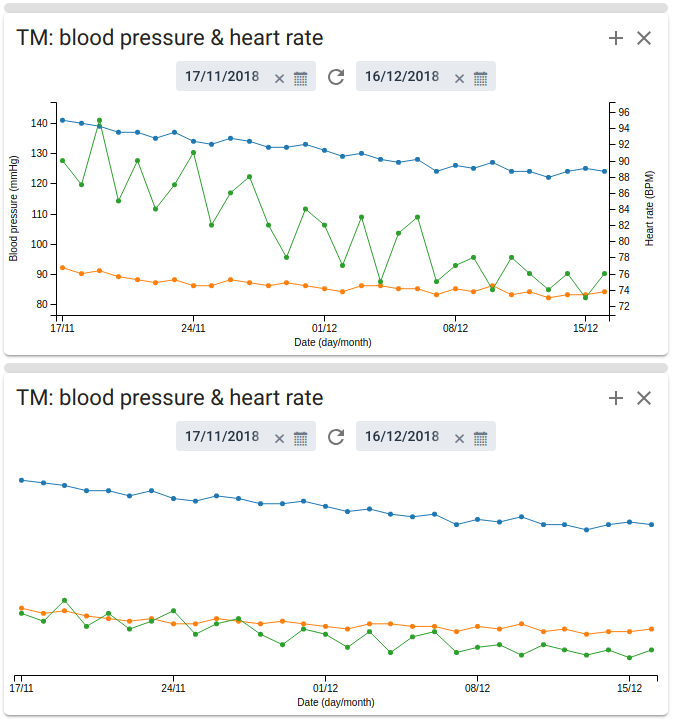
\includegraphics[width=0.8\textwidth]{chapters/4_implementation/tm-compare}
                \caption{The top chart labels both parameters on the y-axis, while the bottom one doesn't.}\label{fig:tm-compare}
            \end{figure}

            The telemonitoring module was the last one to be added to the dashboard. As previously mentioned, C3 was used to plot the data onto a line chart. When the module is added to the dashboard, it will show no data until the user selects the parameters to plot on the chart. This is done by pressing the plus button in the top right corner, which opens a dialog to select the parameters. A maximum of two parameters can be shown on the same chart at a time. In case there are no values for a certain parameter, then the user can't select it. Once a parameter is selected, the user may choose to plot it according to the y-axis. To compare two parameters in relation to each other, it is suggested to plot both these data sets on the y-axis. This normalizes the data on the chart, which in turn makes it easier to compare the data. Figure~\ref{fig:tm-compare} shows the difference. The differences of the green line are in the top chart much more noticeable. However, one can argue that the differences are exaggerated while there is not much difference, which the bottom chart implies.

            Currently, the chart is completely redrawn every time the module changes size. Drawing the chart once and repeatedly resize that one resulted into unexpected behavior where the chart could only grow, but not shrink. Others have reported this on the GitHub page of the library and it is a known issue. As a result the chart is redrawn every time. Thankfully, we did not notice any slowdown. Also, changing the options of the chart will trigger a layout save.

            \begin{figure}[t]
                \centering
                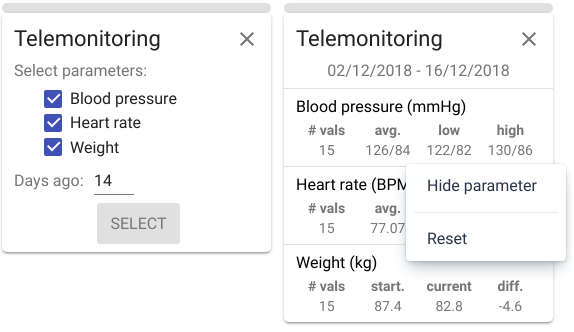
\includegraphics[width=0.7\textwidth]{chapters/4_implementation/tm-small}
                \caption{On the left, the user needs to configure the module. On the right, the summary is shown, together with its context menu.}\label{fig:tm-small}
            \end{figure}

            The small module serves to give a brief summary of all the parameters the user selects for a certain time period. When the module is added, the user must select the parameters to summarize. Also, the user must select a starting date to generate the summary for, by providing the number of days to go back to from today. If the user selects 14, a summary is generated for the data from two weeks ago until today. Once  the module is configured, the layout is saved. To reconfigure the module or hide a parameter, right clicking the parameter will open a context menu. Figure~\ref{fig:tm-small} shows the module. Left on the figure the parameters blood sugar and oxygen are hidden, because there are no data values of those parameters for the current patient. Also, this module can not be resized because the summaries are of fixed height.

	\section{Usability test}\label{usabilitytest}

As the prototype neared completion, a usability test was designed. As the name implies, the purpose of such a test is to assess the usability of a prototype. While the prototype is being tested by a user, the researcher takes note of any usability issues that may arise. This evaluation method results in valuable feedback, as it shows directly how real users use a system~\cite{Nielsen1993}.

In this section we describe the design of a usability test to assess the user experience of the dashboard prototype. This test will focus on the usability aspect of the prototype, and not on the extensibility. However, in the future work section (\ref{future_work}) we give suggestions to test this aspect. All the documents created for the test are found in appendix~\ref{appendix_test_docs}.

    \subsection{Purpose}

    The goal of this test is to evaluate the usability of the dashboard prototype. The modules were designed with the usability principles mentioned in section~\ref{usability} in mind. Customization was added by giving the user more freedom in defining the functionality present in the dashboard. However, the experience of the end-users will determine if this is of added value when used in a clinical setting. Therefore, we are interested in gathering the following information:
    \begin{itemize}
        \item Is the dashboard easy to use? Is there a low or high risk of errors?
        \item Is the dashboard easy to navigate? Are all functions easily found?
        \item Does the dashboard as a whole succeed in displaying information in a clear and concise manner? How about the individual modules?
        \item Is the layout customization practical? Is it fast, slow, error-prone\ldots?
        \item How does the usability of the prototype compare to the system the tester uses?
    \end{itemize}

    \noindent Depending on the answers we receive to these questions, we can determine the next steps to take in future research, mentioned in section~\ref{future_work}. While our primary concern is the evaluation of our prototype, we also want to gain insight on the EHR system(s) the tester uses. This way, we can identify potential improvements or additional features for our prototype going forward. % chktex 36

    \subsection{Participants}\label{test_participants}

    The prototype is designed for use in different medical settings, which are staffed by many different roles. To get the best possible results, we want our group of participants to cover as many different roles as possible. For example, an general care nurse has completely different expectations from an EHR system compared to a paramedic. This will yield feedback we would otherwise not have received if all participants had the same role.

    Therefore, we need variety. Our participants should represent a wide spectrum of the health care industry in terms of the roles they fulfill. On top of that, having participants from different age groups is encouraged. Given the scope of this thesis, we chose the following sectors and roles to gather participants from:
    \begin{itemize}
        \item Laboratory unit: conducting tests and management of lab orders and results.
        \item Intensive care unit: requires close/real-time monitoring of several patients.
        \item General inpatient care: for example non-critical pediatric care within a hospital.
        \item Emergency response: for example a paramedic. Needs to respond fast, handle stressful situations, and needs to be mobile.
        \item A general practitioner: sees many patients daily with a large variety of conditions.
    \end{itemize}

    \noindent Now that we know who we want to test, the next question is how many. Nielsen determined that five participants find almost as much usability problems as for example a group of ten~\cite{Nielsen2012}. In other words, five participants result in the optimal benefit-cost ratio associated with user testing. However, there are exceptions to this rule. A quantitative study for example should test a lot more individuals in order to get statistically significant results.

    Our test is qualitative in nature, since we want to get a deeper understanding of what the needs of the end-user are. We are interested in \emph{why} the user experiences certain things. Therefore, according to Nielsen, we don't need to gather many participants, but preferably still more than five. This is due to the fact that the end-users of the dashboard have different professions and work in different care settings. The needs of each participant vary greatly between these settings, which is why five participants may fall short in uncovering some important usability issues.

    \subsection{Test structure}

    During the recruitment, willing participants may choose when and where the test will take place, given the location will not cause any disturbances. After meeting up, the following procedure takes place, with the estimated time for each step:
    \begin{myenumerate}
        \item Pre-test, 5 to 10 minutes:
        \begin{myenumerate}
            \item Greet and brief the participant.
            \item Ask for informed consent.
            \item The participant fills in a questionnaire which asks for demographic information and information concerning the EHR system he/she currently uses.
        \end{myenumerate}
        \item Test of the dashboard prototype, 20 to 25 minutes:
        \begin{myenumerate}
            \item Give the participant a brief tour of the prototype.
            \item The participant starts following the step-by-plan while being observed. No help or suggestions will be given unless necessary.
        \end{myenumerate}
        \item Post-test, 10 minutes:
        \begin{myenumerate}
            \item The participant fills in a second brief questionnaire about the user experience.
            \item The participant is interviewed. We go over suggestions, what was good/bad, future modules\ldots Additional questions may be asked as the interview goes on.
            \item Debrief the participant and hand out reward.
        \end{myenumerate}
    \end{myenumerate}

    \noindent The informed consent form found in appendix~\ref{appendix_test_consent}, is printed twice and filled in on the spot. The two questionnaires discussed in the next section, were created in Google Forms and are filled in using the laptop which has the prototype installed. Finally, the prototype is tested via the Google Chrome browser. A backup of the database is restored between each test to ensure that every participant will work with the exact same data.

    \subsection{Data gathering}

    The test results in quantitative data from two questionnaires. However, the qualitative information is more important, which is gathered from observing the participant during the test of the prototype and from the interview afterwards. Both questionnaires are found in appendix sections~\ref{appendix_pretest} and~\ref{appendix_posttest}.

    \paragraph{Quantitative data} The first questionnaire asks at the start for demographic information of which the following can be qualified a quantitative data: 
    \vspace{-6pt}
    \begin{myitemize}
        \item Age.
        \item Technology experience (Likert scale, 1: not experienced, 5: experienced).
    \end{myitemize}
    \noindent The second part asks for information regarding the current EHR system that the participant uses: 
    \vspace{-6pt}
    \begin{myitemize}
        \item Satisfaction (Likert scale, 1: very dissatisfied, 5: very satisfied).
        \item User friendliness (Likert scale, 1: strongly disagree, 5: strongly agree).
        \item Supports the participant's needs (Likert scale, 1: strongly disagree, 5: strongly agree).
    \end{myitemize}

    \noindent The second questionnaire asks for ratings regarding the usability of the prototype: 
    \vspace{-6pt}
    \begin{myitemize}
        \item General experience (Likert scale, 1: very bad, 7: very good). Because this is the general opinion of the participant, more steps are defined for this scale.
        \item Easy to use (Likert scale, 1: strongly disagree, 5: strongly agree).
        \item Dashboard looks clean (Likert scale, 1: strongly disagree, 5: strongly agree).
        \item Modules look clean (Likert scale, 1: strongly disagree, 5: strongly agree).
        \item Modules served as a good example (Likert scale, 1: strongly disagree, 5: strongly agree).
        \item Enough customization options present (Likert scale, 1: strongly disagree, 5: strongly agree).
    \end{myitemize}

    \noindent No other quantitative data is gathered. During the observation, errors are noted, but not counted.

    \paragraph{Qualitative data} The bulk of the qualitative data is gathered during the test of the prototype by observation and afterwards during the interview. When the participant is following the step-by-step plan, the following notes may be taken:
    \vspace{-6pt}
    \begin{myitemize}
        \item The participant struggled finding UI element X.
        \item An error was made regarding X.
        \item The participant hesitated at step X.
        \item The participant asked question X regarding Y\ldots
    \end{myitemize}

    \noindent Questions related to the usability of the prototype and the current EHR system, current paper use in their care setting, module suggestions\ldots are asked during the interview. Section~\ref{results_interview} describes what qualitative data was retrieved.

    \subsection{Test procedure}

    During the step-by-step process, the participant works with the dashboard of three fictional patients. A short background is given for each patient and participant performs actions which relate to the situation of the patient. The participant has seen all aspects of the dashboard after the test of the prototype is complete. Appendix~\ref{appendix_test_steps} contains the step-by-step process. Also, the screenshots in appendix~\ref{appendix_test_screens} show the dashboard at the start of each scenario. We now describe each scenario.

    \paragraph{Patient 1} Background: Kenny is an account manager of a large accounting firm. The combination of his stressful job, sedentary lifestyle, and smoking habit have lead to health issues. He has frequent palpitations and high blood pressure. At home, Kenny has to measure his weight, heart rate, and blood pressure on a regular basis with devices that send the values to his electronic patient record. In this scenario the participant does the following:
    \vspace{-6pt}
    \begin{myenumerate}
        \item Apply a filter on the history module.
        \item Add and configure a telemonitoring module to fill the empty space of the dashboard.
        \item Reorder the modules on the summarizing panel, while adding and configuring a small telemonitoring module.
    \end{myenumerate}

    \paragraph{Patient 2} Background: Since Jozefien retired, she has been gaining weight at an alarming rate. As a countermeasure, she regularly visits her general practitioner. Each consultation, the practitioner updates her medication scheme and tells her what she needs to pay attention to. In this scenario the participant does the following:
    \vspace{-6pt}
    \begin{myenumerate}
        \item Remove and add a prescription, check for interactions.
        \item Remove the allergy module to replace it with a workflow module.
        \item Edit some steps of a workflow.
        \item Reset the checklist and add some new tasks to it.
        \item Hide a parameter in the small telemonitoring module found in the left panel.
    \end{myenumerate}

    \paragraph{Patient 3} Background: After a serious car accident, Bert is hospitalized in the intensive care unit. Bert has many allergies, an elaborate medication scheme, and misses some vaccinations. Currently he is being treated by several clinicians and being observed by nurses. It is important that everyone is aware of these allergies, the medication scheme, and missing vaccinations. However, the data in the EHR system is not up to date. The latest most up to date medical data is still stored in a paper dossier. In this scenario the participant does the following:
    \vspace{-16pt}
    \begin{myenumerate}
        \item Change and add an allergy.
        \item Remove and add a vaccination.
        \item Apply a filter on the history module.
    \end{myenumerate}

    \subsection{Recruiting participants}

    The search for participants began immediately after the usability test design was completed. A total of 9 people were contacted with the following backgrounds:
    \vspace{-14pt}
    \begin{myitemize}
        \item 2 nursing students, both had internship experience in a hospital setting.
        \item 1 elderly care nurse.
        \item 2 intensive care unit nurses.
        \item 1 clinical laboratory department head.
        \item 1 paramedic.
        \item 2 home nurses, working for the same practice.
    \end{myitemize}

    \noindent Five individuals immediately were scheduled to test the prototype. The two home nurses and one nursing student declined due to time constraints. The paramedic expressed interest and was scheduled several weeks later. Four general practitioners were contacted, but were unable to participate due to the short notice of the study. Six participants have tested the prototype.

    \subsection{Results}

    Before every test, the database of the application was reset and the log in functionality was tested to avoid any technical problems. As a result, every test ran smoothly without any issues. Every participant tested the prototype in a secluded and silent environment. Four tests were conducted at the homes of the participants and the other two in empty classrooms of Hasselt University. The test was estimated to take approximately 40 minutes to complete. In anticipation of lengthy interviews, a hard stop was put in place should the test pass the 60 minute mark. This was the case for two tests. The durations of the other four were between 45 and 55 minutes. This caused no issues for any of the participants. When the test concluded, participants were rewarded with a bottle of wine. During the recruitment phase, each contacted individual was aware of a reward, but they did not know what it was beforehand. % chktex 1

    \subsubsection{Pre-test questionnaire}

    Table~\ref{table:pre-test} shows some general information from the pre-test questionnaire regarding the participants. It should be noted that 5 out of 6 participants are between the ages 21 and 25. They also indicate a higher familiarity with technology, compared to the older participant. The younger participants also have limited work experience. The pre-test questionnaire also indicated that all participants use their smartphone and lap-/desktop daily. Four participants use their tablet a few times every month, of which one participant uses it daily. One participant uses a smartwatch daily, and is the only one to use a smartwatch at all.
    
    \begin{table}[!t]
        \resizebox{\textwidth}{!}{%
        \begin{tabular}{ccllc}
            \hline % chktex 44
            \textbf{Age} & \textbf{Gender} & \textbf{Profession}        & \textbf{Experience} & \textbf{\begin{tabular}[c]{@{}c@{}}Tech\\ experience (1-5)\end{tabular}} \\ \hline % chktex 44
            21           & M               & Nursing student            & 4 years internship  & 4                                                                  \\
            25           & F               & Elderly care nurse         & 1,5 years           & 4                                                                  \\
            23           & F               & Intensive care unit nurse  & 1 year 5 months     & 4                                                                  \\
            23           & F               & Intensive care unit nurse  & 5 months            & 4                                                                  \\
            49           & F               & Laboratory department head & 28 years            & 3                                                                  \\
            22           & M               & Paramedic                  & 1 year              & 5
        \end{tabular}%
        }
        \caption{Pre-test results: general participant information}\label{table:pre-test}
    \end{table}

    Table~\ref{table:pre-test-ehr} shows that all participants use a different EHR systems for their care setting and only one of them is used on a mobile device. The user satisfaction of the EHR systems scored an average of 4 out 5, with user friendliness scoring a bit less. The participants were more neutral towards the features the EHR system provides, scoring a 3,17 on average. Only two EHR systems provide customization. Lastly, one participant uses no less than 6 applications in combination with the EHR system, while two participants use none. During the interview, more questions were asked concerning their current EHR system.

    \begin{table}[!t]
        \resizebox{\textwidth}{!}{%
        \begin{tabular}{lcccccl}
        \hline
        \textbf{EHR system} & \textbf{Mobile} & \textbf{\begin{tabular}[c]{@{}c@{}}Satisfaction\\ (1-5)\end{tabular}} & \textbf{\begin{tabular}[c]{@{}c@{}}User friendliness\\ (1-5)\end{tabular}} & \textbf{\begin{tabular}[c]{@{}c@{}}Complete\\ toolset (1-5)\end{tabular}} & \textbf{\begin{tabular}[c]{@{}c@{}}Custom-\\ izable\end{tabular}} & \multicolumn{1}{c}{\textbf{\begin{tabular}[c]{@{}c@{}}\# other \\ systems\end{tabular}}} \\ \hline
        Orbis               & No              & 3                                                                     & 3                                                                          & 2                                                                         & No                                                                & 0                                                                                        \\
        GEMS                & No              & 3                                                                     & 3                                                                          & 3                                                                         & No                                                                & 6                                                                                        \\
        Metavision \& GEMS  & No              & 5                                                                     & 4                                                                          & 4                                                                         & No                                                                & 2+                                                                                       \\
        ICCA                & No              & 5                                                                     & 5                                                                          & 4                                                                         & Yes                                                               & 4                                                                                        \\
        HIX                 & No              & 4                                                                     & 4                                                                          & 3                                                                         & Yes                                                               & 1                                                                                        \\
        KWS                 & Yes             & 4                                                                     & 3                                                                          & 3                                                                         & No                                                                & 0
        \end{tabular}%
        }
        \caption{Pre-test results: EHR systems in use by participants. Note: same order is respected as table~\ref{table:pre-test}.}\label{table:pre-test-ehr}
    \end{table}

    \subsubsection{Prototype test: observations}

    All participants were able to complete the test within the allotted time of 20 to 25 minutes. The two intensive care nurses were noticeably faster in completing all the steps, nearing the 15 minute mark. The elderly care nurse and the laboratory head were often unsure on where to click and often asked questions instead of trying. This may explain the fact that they took a bit longer to complete the test compared to the other participants. However, every participant received the same brief tour of the prototype, so no participant had more knowledge of the prototype compared to the others. We now go over the comments made by the participants during the test.

    There were several comments regarding the prescription module. One participant noted that it would be useful if empty dosage fields were automatically filled with zeroes. Currently, the user needs to fill all fields manually. Another participant suggested something similar. Because today's date had to be filled in multiple times throughout the test, the participant would've liked a button that would automatically fill it in. This participant stressed that error checking was a very important component of the systems they currently use. Regarding the end date of prescriptions, one participant noted that they sometimes have to administer medication indefinitely, which the module does not support at the moment. In case there are interactions between medicines, one participant noted that it would be helpful to see the actual interaction effects in addition to the interacting medicine.

    The test highlighted two issues. First, four participants struggled to add a new task to the checklist. This was done by opening the context menu on top of the checklist description. In this case, a button would be a better option. Second, three participants had difficulties finding the option to add a vaccination entry, which again was found in a context menu. More careful thought must be given on when to use these context menus. However, one participant had no issues with the context menu and thought it was really useful. This participant shared this thought also for the date picker.

    Participants had a few more comments. Instead of clicking the arrow button to open the dashboard of a patient, the user can click anywhere in the row of the table to open it. Also, one participant liked both the normal and small telemonitoring modules in particular, describing them as very clean and simple. To conclude, a participant described the importance of access control and privacy surrounding the patient data history module. 
    
    \subsubsection{Post-test questionnaire}

    Table~\ref{table:post-test} shows the results of the Likert scale questions concerning the usability of the prototype. The results are very positive, indicating a good overall experience with the dashboard. Furthermore, all participants indicated that they had no trouble finding their way around the dashboard. However, these results are not conclusive, due to the small sample size. Also, the fifth participant was the only older person in the sample group. The general experience of the dashboard and the experience with technology were both lower for this participant. But then again, a laboratory setting does not share many similarities with the other settings found in the sample group. 
    
    Maybe the most important result is that the modules served as good examples of what is possible with the dashboard. This allowed the participants to better relate the prototype to their work setting, which may lead to valuable feedback during the interview. Also, the questionnaire asked the participants to suggest some modules which would fit the dashboard, which we discuss in more detail in the next section.

    \begin{table}[!t]
        \resizebox{\textwidth}{!}{%
        \begin{tabular}{cccccc}
        \hline
        \textbf{\begin{tabular}[c]{@{}c@{}}General\\ experience\\ (1-7)\end{tabular}} & \textbf{\begin{tabular}[c]{@{}c@{}}Ease\\ of use\\ (1-5)\end{tabular}} & \textbf{\begin{tabular}[c]{@{}c@{}}Dashboard\\ clear UI\\ (1-5)\end{tabular}} & \textbf{\begin{tabular}[c]{@{}c@{}}Modules\\ clear UI\\ (1-5)\end{tabular}} & \multicolumn{1}{l}{\textbf{\begin{tabular}[c]{@{}l@{}}Modules good\\ examples (1-5)\end{tabular}}} & \textbf{\begin{tabular}[c]{@{}c@{}}Enough\\ Customization\\ (1-5)\end{tabular}} \\ \hline
        6                                                                             & 5                                                                      & 5                                                                             & 5                                                                           & 4                                                                                                  & 5                                                                               \\
        6                                                                             & 4                                                                      & 3                                                                             & 4                                                                           & 4                                                                                                  & 4                                                                               \\
        6                                                                             & 4                                                                      & 5                                                                             & 4                                                                           & 5                                                                                                  & 5                                                                               \\
        7                                                                             & 5                                                                      & 5                                                                             & 5                                                                           & 5                                                                                                  & 5                                                                               \\
        4                                                                             & 3                                                                      & 4                                                                             & 4                                                                           & 4                                                                                                  & 4                                                                               \\
        7                                                                             & 5                                                                      & 5                                                                             & 5                                                                           & 5                                                                                                  & 5                                                                               \\ \hline
        \textbf{6}                                                                    & \textbf{4,33}                                                          & \textbf{4,5}                                                                  & \textbf{4,5}                                                                & \textbf{4,5}                                                                                       & \textbf{4,67}                                                                   \\ \hline
        \end{tabular}%
        }
        \caption{Post-test results: questionnaire to assess usability of the dashboard. The bottom row indicates the average scores. Note: same order is respected as table~\ref{table:pre-test}.}\label{table:post-test}
    \end{table}

    \subsubsection{Interview}\label{results_interview}

    Several topics were brought up during the interview, such as potential modules to add to the dashboard, use cases for the current modules, the current EHR system that is in use, the existence of paper in the work setting, what was good or bad, and other suggestions. For each topic, we discuss the feedback the participants gave us.

    \paragraph{Module suggestions} Two participants suggested a drip management module. A drip, or intravenous therapy, is the administration of a fluid solution directly into a vein. This is often done via syringes. The module would help regulate and track the volume of the drip. Also, if the drip administers a medicine which affects blood pressure, then the module tracks this parameter as well. In case something is unusual is happening to this parameter, the module alerts the caregivers. This module is much more practical than managing the drips of multiple patients the manual way. A computer can easily track many ongoing drips.

    Another module was suggested twice. Fluid balance is the balance between fluid that enters the body and fluid that leaves the body. This closely relates to drips, which serves as fluid input. A fluid balance module helps tracking the amount of fluid that enters and leaves a patient's body. In case any abnormalities occur, then the module can notify the clinician. This again is an example how these systems can automate several steps of these processes.

    Wound management is tedious process, as no wound is the same. A cut needs to be treated different than a stab from a needle. There exists a large variety of these wounds that each have their own step-by-step guide to treat them. A wound management module can provide the right guide at the right time. This way clinicians don't need to search through a thick file. Also, a participant suggested that if the module was used on a smartphone, the camera can be used to take pictures of the wound.

    A participant also suggested an emergency contact module. For example, this module contains information of the family members of the patient. But it may also contain the contact information of the doctor on night duty. Since these doctors rotate their night shift periodically, it takes time look up the information manually via a paper calendar. If this again was used on a mobile phone, calls can be directly initiated from the module.

    Other suggestions included body temperature monitoring, diabetes management, diet management, and pain status or relief modules. However, the previously mentioned ones were thoroughly explained by the participants on how they would see it being used in practice. One participant suggested a notification hub. This would be very beneficial for the dashboard, but also difficult to realize. A notification hub is not a module, but it is deeply rooted in the architecture of the application. From our approach, all integrated modules need to have a standardized way to implement the firing of notifications.

    \paragraph{Use cases current modules}

    Every participant was asked if they could devise a scenario in which they would use the dashboard or a module from it. This resulted in several use cases, in particular to the workflow and checklist modules. Where one participant mentioned wound management as a potential module, another participant would use the workflow module to do this. In this case, every specific wound represents a workflow. 
    
    Another participant mentioned that every operation leads to a specific care path that needs to be followed. The participant saw this as an opportunity to model these paths in the workflow module. Furthermore, another workflow use case was to store patient specific requests in there. The participant gave following example: ``An elderly lady wants to visit the chapel of the hospital every Sunday morning. However, she may not go alone and someone needs to accompany her.'' The workflow module serves as a reminder tool in this case.

    If the workflow module allowed branching in the form of ``if A happens, do B, else C'', then a lot more possible use cases would arise, according to a participant. Another suggestion was to extend the patient information module by logging the ``Do Not Resuscitate'' order, or in other words, allow natural death to occur. To conclude, the checklist module also generated some use cases, such as: record the current administered medications, log the steps of the morning care routine, checking of parameters, and wound management.

    \paragraph{Current EHR system}

    Four out of six participants mentioned that their current system is not customizable. When the other two participants were asked to clarify the customization aspect in their EHR system, they both mentioned that ``a doctor gets a very different layout compared to mine'' and that the IT staff listens to their feedback. This is not what we meant by customization, which turned out to be limited in those two systems as well.

    Some participants used a few software packages next to their EHR system. For one participant, the functions of these extra software packages were as follows: a consultation and transportation planner for patients, a diet planner which was connected to the catering service, and a support service for technical issues. One participant noted that next to their EHR system, they used a software package to retrieve lab results and send lab orders. When taking blood samples, these had to be recorded in both applications, which seemed useless to the participant.

    Several other issues were highlighted regarding the current EHR systems. In one case, the system changes often, which causes it to break occasionally. Also, whenever an external digital document was received, the records it contained needed to be entered manually into the EHR system. Another participant highlighted that the system required a significant amount of training and that the application was not easy to use.

    Lastly, a participant emphasized the fine-grained privacy rules and access control measures that were in place in their system. However, this resulted in some cases that there was no access to a medical record when there should be, hindering care delivery. The participant concluded that striking a balance between data availability and strict privacy rules is a difficult subject for such software. Another participant noted that the EHR system gave away too much information, thinking that they should not be able to see some pieces of information.

    \paragraph{Paper usage}

    Generally, paper usage was fairly limited for all participants. The intensive care nurses used no paper for internal care delivery. However, lab, prescription, and imaging orders were transferred on paper to other departments. The laboratory manager does not use any paper anymore since the latest upgrade of their EHR system. One participant mentioned that the administered medication for patients was still written down on paper, which seems troubling.

    To conclude, one participant made the interesting comparison of paper usage with the use of laptop carts. These carts make it possible for clinicians to have more mobility in terms of computer access. However, the participant noted that these carts would get lost or get in the way, and wanted a truly mobile solution such as tablet computers. This participant noted as well that tablets may solve some other inefficiencies. When recording health parameters of patients, then the clinicians might be required out of protocol to immediately enter the data into the digital system. This results in a lot of walking from room to room which can be avoided by having a mobile device available to directly record the data with.
    
    \paragraph{General}

    One participant described that the customization aspect will be helpful to remind the clinician with what patient they are dealing with. Currently, the same layout is displayed for each patient, which may lead to confusion during a high workload. However, the same participant and another one, felt that the customization would be a lot of work for patients that wont stay long. A solution for this, suggested by three participants in total, was to provide default module configurations, either provided by the system or created by the clinician. One participant mentioned that it should be possible to prohibit the removal of some modules that are absolutely necessary in a given setting. The laboratory manager did not see the added benefit of customization in their work setting. Mainly, because their workflow does not frequently change, and because the software they currently use is very satisfactory.

	\section{Discussion}\label{discussion}

The search for participants began immediately after the usability test design was completed. This section describes the recruitment process, whereafter the results of the usability tests are noted.

    \subsection{Recruiting participants}

    A total of 9 people were contacted with the following backgrounds:
    \vspace{-6pt}
    \begin{myitemize}
        \item 2 nursing students, both had internship experience in a hospital setting.
        \item 1 elderly care nurse.
        \item 2 intensive care unit nurses.
        \item 1 clinical laboratory department head.
        \item 1 paramedic.
        \item 2 home nurses, working for the same practice.
    \end{myitemize}

    \noindent Five individuals immediately were scheduled to test the prototype. The two home nurses and one nursing student declined due to time constraints. The paramedic expressed interest but was unreachable for two weeks until the start of the new year. Four general practitioners were contacted, but were unable to participate due to the short notice of the study. Six participants have tested the prototype.

    \subsection{Results}

    Before every test, the database of the application was reset and the log in functionality was tested to avoid any technical problems. As a result, every test ran smoothly without any issues. Every participant tested the prototype in a secluded and silent environment. Four tests were conducted at the homes of the participants and the other two in empty classrooms of Hasselt University. The test was estimated to take approximately 40 minutes to complete. In anticipation of lengthy interviews, a hard stop was put in place should the test pass the 60 minute mark. This was the case for two tests. The durations of the other four were between 45 and 55 minutes. This caused no issues for any of the participants. When the test concluded, participants were rewarded with a bottle of wine. During the recruitment phase, each contacted individual was aware of a reward, but they did not know what it was beforehand. % chktex 1

    \subsubsection{Pre-test questionnaire}

    Table~\ref{table:pre-test} shows some general information from the pre-test questionnaire regarding the participants. It should be noted that 5 out of 6 participants are between the ages 21 and 25. They also indicate a higher familiarity with technology, compared to the older participant. The younger participants also have limited work experience. The pre-test questionnaire also indicated that all participants use their smartphone and lap-/desktop daily. Four participants use their tablet a few times every month, of which one participant uses it daily. One participant uses a smartwatch daily, and is the only one to use a smartwatch at all.
    
    \begin{table}[!t]
        \resizebox{\textwidth}{!}{%
        \begin{tabular}{ccllc}
            \hline % chktex 44
            \textbf{Age} & \textbf{Gender} & \textbf{Profession}        & \textbf{Experience} & \textbf{\begin{tabular}[c]{@{}c@{}}Tech\\ experience (1-5)\end{tabular}} \\ \hline % chktex 44
            21           & M               & Nursing student            & 4 years internship  & 4                                                                  \\
            25           & F               & Elderly care nurse         & 1,5 years           & 4                                                                  \\
            23           & F               & Intensive care unit nurse  & 1 year 5 months     & 4                                                                  \\
            23           & F               & Intensive care unit nurse  & 5 months            & 4                                                                  \\
            49           & F               & Laboratory department head & 28 years            & 3                                                                  \\
            22           & M               & Paramedic                  & 1 year              & 5
        \end{tabular}%
        }
        \caption{Pre-test results: general participant information}\label{table:pre-test}
    \end{table}

    Table~\ref{table:pre-test-ehr} shows that all participants use a different EHR systems for their care setting and only one of them is used on a mobile device. The user satisfaction of the EHR systems scored an average of 4 out 5, with user friendliness scoring a bit less. The participants were more neutral towards the features the EHR system provides, scoring a 3,17 on average. Only two EHR systems provide customization. Lastly, one participant uses no less than 6 applications in combination with the EHR system, while two participants use none. During the interview, more questions were asked concerning their current EHR system.

    \begin{table}[!t]
        \resizebox{\textwidth}{!}{%
        \begin{tabular}{lcccccl}
        \hline
        \textbf{EHR system} & \textbf{Mobile} & \textbf{\begin{tabular}[c]{@{}c@{}}Satisfaction\\ (1-5)\end{tabular}} & \textbf{\begin{tabular}[c]{@{}c@{}}User friendliness\\ (1-5)\end{tabular}} & \textbf{\begin{tabular}[c]{@{}c@{}}Complete\\ toolset (1-5)\end{tabular}} & \textbf{\begin{tabular}[c]{@{}c@{}}Custom-\\ izable\end{tabular}} & \multicolumn{1}{c}{\textbf{\begin{tabular}[c]{@{}c@{}}\# other \\ systems\end{tabular}}} \\ \hline
        Orbis               & No              & 3                                                                     & 3                                                                          & 2                                                                         & No                                                                & 0                                                                                        \\
        GEMS                & No              & 3                                                                     & 3                                                                          & 3                                                                         & No                                                                & 6                                                                                        \\
        Metavision \& GEMS  & No              & 5                                                                     & 4                                                                          & 4                                                                         & No                                                                & 2+                                                                                       \\
        ICCA                & No              & 5                                                                     & 5                                                                          & 4                                                                         & Yes                                                               & 4                                                                                        \\
        HIX                 & No              & 4                                                                     & 4                                                                          & 3                                                                         & Yes                                                               & 1                                                                                        \\
        KWS                 & Yes             & 4                                                                     & 3                                                                          & 3                                                                         & No                                                                & 0
        \end{tabular}%
        }
        \caption{Pre-test results: EHR systems in use by participants. Note: same order is respected as table~\ref{table:pre-test}.}\label{table:pre-test-ehr}
    \end{table}

    \subsubsection{Prototype test: observations}

    All participants were able to complete the test within the allotted time of 20 to 25 minutes. The two intensive care nurses were noticeably faster in completing all the steps, nearing the 15 minute mark. The elderly care nurse and the laboratory head were often unsure on where to click and often asked questions instead of trying. This may explain the fact that they took a bit longer to complete the test compared to the other participants. However, every participant received the same brief tour of the prototype, so no participant had more knowledge of the prototype compared to the others. We now go over the comments made by the participants during the test.

    There were several comments regarding the prescription module. One participant noted that it would be useful if empty dosage fields were automatically filled with zeroes. Currently, the user needs to fill all fields manually. Another participant suggested something similar. Because today's date had to be filled in multiple times throughout the test, the participant would've liked a button that would automatically fill it in. This participant stressed that error checking was a very important component of the systems they currently use. Regarding the end date of prescriptions, one participant noted that they sometimes have to administer medication indefinitely, which the module does not support at the moment. In case there are interactions between medicines, one participant noted that it would be helpful to see the actual interaction effects in addition to the interacting medicine.

    The test highlighted two issues. First, four participants struggled to add a new task to the checklist. This was done by opening the context menu on top of the checklist description. In this case, a button would be a better option. Second, three participants had difficulties finding the option to add a vaccination entry, which again was found in a context menu. More careful thought must be given on when to use these context menus. However, one participant had no issues with the context menu and thought it was really useful. This participant shared this thought also for the date picker.

    Participants had a few more comments. Instead of clicking the arrow button to open the dashboard of a patient, the user can click anywhere in the row of the table to open it. Also, one participant liked both the normal and small telemonitoring modules in particular, describing them as very clean and simple. To conclude, a participant described the importance of access control and privacy surrounding the patient data history module. 
    
    \subsubsection{Post-test questionnaire}

    Table~\ref{table:post-test} shows the results of the Likert scale questions concerning the usability of the prototype. The results are very positive, indicating a good overall experience with the dashboard. Furthermore, all participants indicated that they had no trouble finding their way around the dashboard. However, these results are not conclusive, due to the small sample size. Also, the fifth participant was the only older person in the sample group. The general experience of the dashboard and the experience with technology were both lower for this participant. But then again, a laboratory setting does not share many similarities with the other settings found in the sample group. 
    
    Maybe the most important result is that the modules served as good examples of what is possible with the dashboard. This allowed the participants to better relate the prototype to their work setting, which may lead to valuable feedback during the interview. Also, the questionnaire asked the participants to suggest some modules which would fit the dashboard, which we discuss in more detail in the next section.

    \begin{table}[!t]
        \resizebox{\textwidth}{!}{%
        \begin{tabular}{cccccc}
        \hline
        \textbf{\begin{tabular}[c]{@{}c@{}}General\\ experience\\ (1-7)\end{tabular}} & \textbf{\begin{tabular}[c]{@{}c@{}}Ease\\ of use\\ (1-5)\end{tabular}} & \textbf{\begin{tabular}[c]{@{}c@{}}Dashboard\\ clear UI\\ (1-5)\end{tabular}} & \textbf{\begin{tabular}[c]{@{}c@{}}Modules\\ clear UI\\ (1-5)\end{tabular}} & \multicolumn{1}{l}{\textbf{\begin{tabular}[c]{@{}l@{}}Modules good\\ examples (1-5)\end{tabular}}} & \textbf{\begin{tabular}[c]{@{}c@{}}Enough\\ Customization\\ (1-5)\end{tabular}} \\ \hline
        6                                                                             & 5                                                                      & 5                                                                             & 5                                                                           & 4                                                                                                  & 5                                                                               \\
        6                                                                             & 4                                                                      & 3                                                                             & 4                                                                           & 4                                                                                                  & 4                                                                               \\
        6                                                                             & 4                                                                      & 5                                                                             & 4                                                                           & 5                                                                                                  & 5                                                                               \\
        7                                                                             & 5                                                                      & 5                                                                             & 5                                                                           & 5                                                                                                  & 5                                                                               \\
        4                                                                             & 3                                                                      & 4                                                                             & 4                                                                           & 4                                                                                                  & 4                                                                               \\
        7                                                                             & 5                                                                      & 5                                                                             & 5                                                                           & 5                                                                                                  & 5                                                                               \\ \hline
        \textbf{6}                                                                    & \textbf{4,33}                                                          & \textbf{4,5}                                                                  & \textbf{4,5}                                                                & \textbf{4,5}                                                                                       & \textbf{4,67}                                                                   \\ \hline
        \end{tabular}%
        }
        \caption{Post-test results: questionnaire to assess usability of the dashboard. The bottom row indicates the average scores. Note: same order is respected as table~\ref{table:pre-test}.}\label{table:post-test}
    \end{table}

    \subsubsection{Interview}

    Several topics were brought up during the interview, such as potential modules to add to the dashboard, use cases for the current modules, the current EHR system that is in use, the existence of paper in the work setting, what was good or bad, and other suggestions. For each topic, we discuss the feedback the participants gave us.

    \paragraph{Module suggestions} Two participants suggested a drip management module. A drip, or intravenous therapy, is the administration of a fluid solution directly into a vein. This is often done via syringes. The module would help regulate and track the volume of the drip. Also, if the drip administers a medicine which affects blood pressure, then the module tracks this parameter as well. In case something is unusual is happening to this parameter, the module alerts the caregivers. This module is much more practical than managing the drips of multiple patients the manual way. A computer can easily track many ongoing drips.

    Another module was suggested twice. Fluid balance is the balance between fluid that enters the body and fluid that leaves the body. This closely relates to drips, which serves as fluid input. A fluid balance module helps tracking the amount of fluid that enters and leaves a patient's body. In case any abnormalities occur, then the module can notify the clinician. This again is an example how these systems can automate several steps of these processes.

    Wound management is tedious process, as no wound is the same. A cut needs to be treated different than a stab from a needle. There exists a large variety of these wounds that each have their own step-by-step guide to treat them. A wound management module can provide the right guide at the right time. This way clinicians don't need to search through a thick file. Also, a participant suggested that if the module was used on a smartphone, the camera can be used to take pictures of the wound.

    A participant also suggested an emergency contact module. For example, this module contains information of the family members of the patient. But it may also contain the contact information of the doctor on night duty. Since these doctors rotate their night shift periodically, it takes time look up the information manually via a paper calendar. If this again was used on a mobile phone, calls can be directly initiated from the module.

    Other suggestions included body temperature monitoring, diabetes management, diet management, and pain status or relief modules. However, the previously mentioned ones were thoroughly explained by the participants on how they would see it being used in practice. One participant suggested a notification hub. This would be very beneficial for the dashboard, but also difficult to realize. A notification hub is not a module, but it is deeply rooted in the architecture of the application. From our approach, all integrated modules need to have a standardized way to implement the firing of notifications.

    \paragraph{Use cases current modules}

    Every participant was asked if they could devise a scenario in which they would use the dashboard or a module from it. This resulted in several use cases, in particular to the workflow and checklist modules. Where one participant mentioned wound management as a potential module, another participant would use the workflow module to do this. In this case, every specific wound represents a workflow. 
    
    Another participant mentioned that every operation leads to a specific care path that needs to be followed. The participant saw this as an opportunity to model these paths in the workflow module. Furthermore, another workflow use case was to store patient specific requests in there. The participant gave following example: ``An elderly lady wants to visit the chapel of the hospital every Sunday morning. However, she may not go alone and someone needs to accompany her.'' The workflow module serves as a reminder tool in this case.

    If the workflow module allowed branching in the form of ``if A happens, do B, else C'', then a lot more possible use cases would arise, according to a participant. Another suggestion was to extend the patient information module by logging the ``Do Not Resuscitate'' order, or in other words, allow natural death to occur. To conclude, the checklist module also generated some use cases, such as: record the current administered medications, log the steps of the morning care routine, checking of parameters, and wound management.

    \paragraph{Current EHR system}

    Four out of six participants mentioned that their current system is not customizable. When the other two participants were asked to clarify the customization aspect in their EHR system, they both mentioned that ``a doctor gets a very different layout compared to mine'' and that the IT staff listens to their feedback. This is not what we meant by customization, which turned out to be limited in those two systems as well.

    Some participants used a few software packages next to their EHR system. For one participant, the functions of these extra software packages were as follows: a consultation and transportation planner for patients, a diet planner which was connected to the catering service, and a support service for technical issues. One participant noted that next to their EHR system, they used a software package to retrieve lab results and send lab orders. When taking blood samples, these had to be recorded in both applications, which seemed useless to the participant.

    Several other issues were highlighted regarding the current EHR systems. In one case, the system changes often, which causes it to break occasionally. Also, whenever an external digital document was received, the records it contained needed to be entered manually into the EHR system. Another participant highlighted that the system required a significant amount of training and that the application was not easy to use.

    Lastly, a participant emphasized the fine-grained privacy rules and access control measures that were in place in their system. However, this resulted in some cases that there was no access to a medical record when there should be, hindering care delivery. The participant concluded that striking a balance between data availability and strict privacy rules is a difficult subject for such software. Another participant noted that the EHR system gave away too much information, thinking that they should not be able to see some pieces of information.

    \paragraph{Paper usage}

    Generally, paper usage was fairly limited for all participants. The intensive care nurses used no paper for internal care delivery. However, lab, prescription, and imaging orders were transferred on paper to other departments. The laboratory manager does not use any paper anymore since the latest upgrade of their EHR system. One participant mentioned that the administered medication for patients was still written down on paper, which seems troubling.

    To conclude, one participant made the interesting comparison of paper usage with the use of laptop carts. These carts make it possible for clinicians to have more mobility in terms of computer access. However, the participant noted that these carts would get lost or get in the way, and wanted a truly mobile solution such as tablet computers. This participant noted as well that tablets may solve some other inefficiencies. When recording health parameters of patients, then the clinicians might be required out of protocol to immediately enter the data into the digital system. This results in a lot of walking from room to room which can be avoided by having a mobile device available to directly record the data with.
    
    \paragraph{General}

    One participant described that the customization aspect will be helpful to remind the clinician with what patient they are dealing with. Currently, the same layout is displayed for each patient, which may lead to confusion during a high workload. However, the same participant and another one, felt that the customization would be a lot of work for patients that wont stay long. A solution for this, suggested by three participants in total, was to provide default module configurations, either provided by the system or created by the clinician. One participant mentioned that it should be possible to prohibit the removal of some modules that are absolutely necessary in a given setting. The laboratory manager did not see the added benefit of customization in their work setting. Mainly, because their workflow does not frequently change, and because the software they currently use is very satisfactory.

	\section{Conclusion and future work}

The results of the usability test led to valuable feedback. However, it also highlighted the shortcomings of this study. The last step of this work was to take a critical look at the end result of the entire thesis. From this we draw several conclusions, which lead to interesting topics for future work.

    \subsection{Conclusion}

    The literature study brought the following issues caused by EHR systems to light:
    \begin{myitemize}
        \item An increase in the medical error rate after the installation of an EHR system, caused by poor usability and paper workarounds for missing functions.
        \item Heavy workflow disruption caused by the adoption or the update process of the system, resulting in productivity loss and negative motions.
    \end{myitemize}

    \noindent The design of the dashboard put a heavy focus on both usability and interoperability to resolve these issues. The test indicated that the dashboard had good usability. This partly resolves the first issue. The dashboard application was also easy to learn. As a result, clinicians adapt quickly to the new system, limiting a loss in productivity. Also, the good usability of the dashboard facilitates a positive user experience. It seems this resolves the second issue, which is not the case.

    The usability test featured a simple version of the dashboard, not suitable for deployment in a care setting. Therefore, the test can not measure whether these two issues are resolved. This requires a clinical trial wherein the prototype is tested in a real clinical setting. The issues arise only for these scenarios. However, clinical trials are complex studies and often require a prototype that closely resembles the final product. Also, real patient data is involved which requires security and privacy measurements to be in place. We discuss clinical trials later on.

    Another test needs to be designed to assess the interoperability aspect of the prototype and how it solves the two problems. Such a test requires the IT staff of an institution to integrate and change several components that possibly interrupt the workflow of clinicians. This also evaluates the base components and the MVC architecture.

    The last paragraphs indicate the shortcomings of the study. However, the prototype was received very well by the test participants. The feedback from the usability test, together with the insights gained during development, brought forth an extensive collection of future improvements and ideas. We conclude the thesis by providing a list of interesting topics for future research.

    \subsection{Future work}\label{future_work}

    In this section, we present a list of topics that future research may focus on. We go into more detail on some of these by indicating, for example, the requirements, the goals, and the process. All the topics are related to each other are mentioned in no particular order.
 
    % grand scheme
    % plan test
    % plan developer test
    \subsubsection{Clinical trial}

    Clinical trials are used to generate data on safety, efficacy, and/or effectiveness of treatments~\cite{Minneci2018}. The design and implementation of clinical trials is challenging, but they are necessary to improve health care. Before the trial may start, approval is needed from an ethics committee of the country wherein it will take place. A clinical trial needs a more advanced prototype of the dashboard compared to the one developed here. It should already have some security and privacy measures in place. Also, the prototype should feature more advanced components that are suitable for the testing environment.

    Assume the following scenario where we have built an advanced prototype. At the first stage of a clinical trial, this is tested by a small group of users. The gathered feedback is then implemented in the next version of the prototype. The new version is tested again, but by a larger sample group. This cycle repeats a few times. At a certain stage, the prototype is tested by hundreds of users. This indicates that clinical trials can be very costly. Therefore, a clinical trial for the dashboard application is not for the near future.

    \subsubsection{Evaluate effect of interoperability}

    The evaluation of the interoperability aspect requires two different tests. The benefits of the module-based approach mentioned in section~\ref{proposal} should minimize the loss in productivity due to workflow disruption. This requires a testing environment where such disruptions happen, which is difficult to control. Therefore, the prototype should repeatedly lead to positive results. Also, the test requires the prototype to be advanced enough to support the testing environment under normal conditions. The clinical trial of the dashboard prototype can include this test.

    A second test involves the IT staff of a health care institution. The goal of this test is to evaluate the integration of new modules into the dashboard. The effect this has on workflow disruption needs to be thoroughly observed during the test. Again, this is a difficult environment to control. The feedback we receive from the IT staff will help to improve the base components and the back end structure.
    
    \subsubsection{Prototype improvement}

    The prototype can be improved on two levels: on a dashboard level, and on a module level. Dashboard improvements relate to changes that affect the entire dashboard, while module improvements only change the inner workings of a certain module. 
    
    \paragraph{Dashboard improvements} Currently, clinicians can create a custom dashboard for each patient. In the future, every clinician has one personal dashboard. This dashboard can contain other modules which are only of use to the caregiver. It may be filled with shortcuts to patients, an agenda, a personal routine, and more. Examples of modules for this type of dashboard were already uncovered during the brainstorm session in section~\ref{module_brainstorm}.

    One participant wished for a notification module in the prototype. This module gathers all the notifications that modules or the dashboard sends. To support this, the base components need to be updated so modules can override a function which creates the notification. Also, two participants suggested that the dashboard should provide default layouts which are also editable. It should also be possible to mark modules of layouts as necessary, to prevent them from being removed. Sometimes a module is absolutely necessary in a certain workflow.

    \paragraph{Module improvements} The base components need to be updated to support notifications. It should help the modules define their own notifications according to the template the base component defines. Also, modules should be able to show or hide certain data according to its size. This removes the need for the small component definitions, because a small sized normal module will look the same.

    Test participants suggested several modules. A wound management module would serve as a collection of steps to treat many different wounds. This removes the need for ring binders, which are difficult to search through. A drip management module was also suggested. This module helps the tracking of the drips of many patients. It may provide suggestions based on the vital signs of the patient and the currently configured drip. Finally, a fluid balance module helps tracking the fluid intake and output of a patient. The intake should include the same information of the drips managed with the previous module. During the clinical trial, many more useful modules may come to light.


    %% dashboard specific
    %% module specific

    \newpage
\appendix

\section{Appendix}

\subsection{Low fidelity prototypes} \label{app_low_fidelity}

\begin{figure}[!htb]
    \centering
    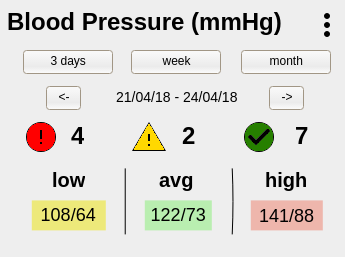
\includegraphics[width=0.45\textwidth]{chapters/3_design/mockups/bp_small}
    \caption{Small blood pressure module}\label{fig:bp_small}
\end{figure}

\begin{figure}[!htb]
    \centering
    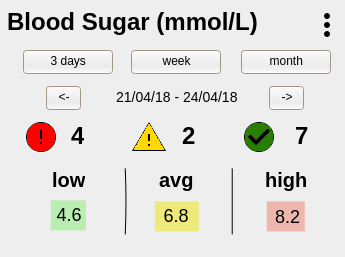
\includegraphics[width=0.45\textwidth]{chapters/3_design/mockups/bs_small}
    \caption{Small blood sugar module}\label{fig:bs_small}
\end{figure}

\begin{figure}[!htb]
    \centering
    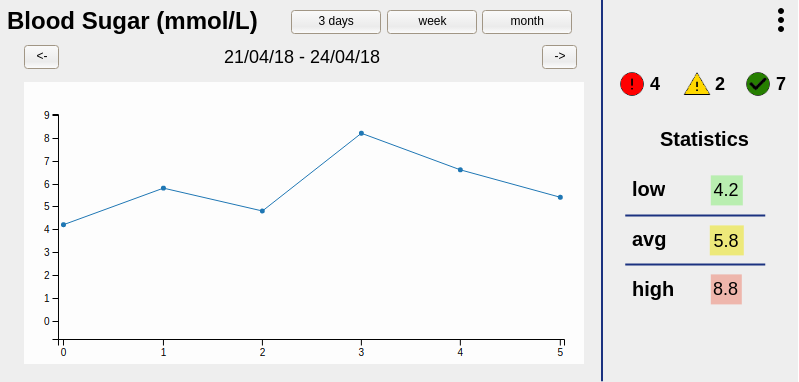
\includegraphics[width=0.75\textwidth]{chapters/3_design/mockups/bs_large}
    \caption{Large blood sugar module}\label{fig:bs_large}
\end{figure}

\begin{figure}[!htb]
    \centering
    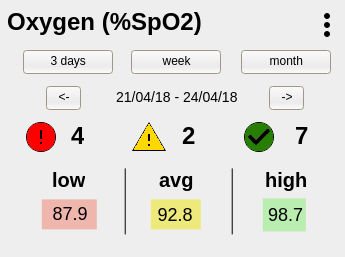
\includegraphics[width=0.45\textwidth]{chapters/3_design/mockups/oxygen_small}
    \caption{Small oxygen module}\label{fig:oxygen_small}
\end{figure}

\begin{figure}[!htb]
    \centering
    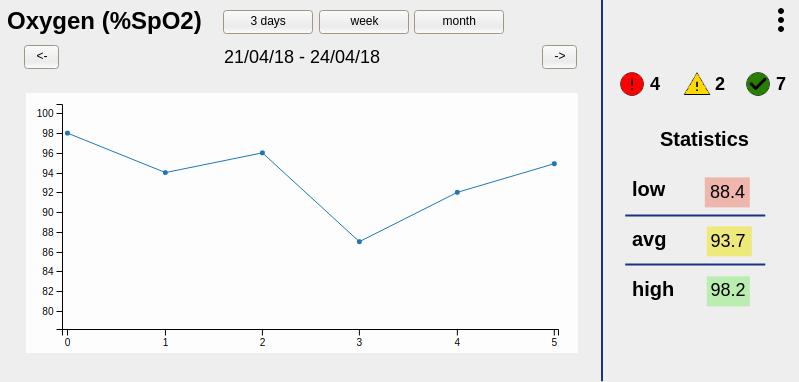
\includegraphics[width=0.75\textwidth]{chapters/3_design/mockups/oxygen_large}
    \caption{Large oxygen module}\label{fig:oxygen_large}
\end{figure}

\clearpage
\subsection{REST API documentation} \label{app_rest_api}

    \subsubsection{User}

        The user module was created to show basic information and does not offer much functionality.

        \paragraph{Create user} Creates a new user in the database.
        \begin{itemize}
            \item \textbf{URL}: /user
            \item \textbf{Method}: \texttt{POST}
            \item \textbf{Data Params}: \begin{verbatim}
    {
        "firstName": "John",
        "lastName": "Doe",
        "birth": "1998-09-15T15:53:00",
        "gender": "M",
        "bloodType": "O+",
        "height": "1.77m",
        "address": "Agoralaan, 3590 Diepenbeek",
        "phone": "0123/456789"
    }
            \end{verbatim}
        \end{itemize}

        \paragraph{Get user} Get the information of a user according to the supplied id.
        \begin{itemize}
            \item \textbf{URL}: /user/:id
            \item \textbf{Method}: \texttt{GET}
            \item \textbf{URL Params}: \texttt{id=[string]}
            \item \textbf{Response}: \begin{verbatim}
    {
        "_id": "5b5c65e3ad30264506380dd1",
        "firstName": "John",
        "lastName": "Doe",
        "birth": "2008-09-15T15:53:00",
        "gender": "M","bloodType": "O+",
        "height": "1.77m",
        "address": "Agoralaan, 3590 Diepenbeek",
        "phone": "0123/456789"
    }
            \end{verbatim}
        \end{itemize}

    \subsubsection{Blood pressure}

        \paragraph{Get blood pressure values for large module} Get blood pressure values within given period.
        \begin{itemize}
            \item \textbf{URL}: /bp/:start\&:end
            \item \textbf{Method}: \texttt{GET}
            \item \textbf{URL Params}: \texttt{start=[integer], end=[integer]}
            \item \textbf{Response}: \begin{verbatim}
    {
        "thresholds": Object,
        "values": Array,
        "avgLine": Array // contains info to draw 
    }                    // average lines on chart
            \end{verbatim}
        \end{itemize}

        \paragraph{Get blood pressure statistics for small module} Get blood pressure statistics within given period.
        \begin{itemize}
            \item \textbf{URL}: /bp/small/:start\&:end
            \item \textbf{Method}: \texttt{GET}
            \item \textbf{URL Params}: \texttt{start=[integer], end=[integer]}
            \item \textbf{Response}: \begin{verbatim}
    {
        "low": "110/68",
        "high": "131/88",
        "avg": "119.7/78.0",
        "dangerVals": 1,
        "warningVals": 1,
        "okVals": 1,
        "lowCol": "yellow",
        "avgCol": "green",
        "highCol": "red",
        "thresholds": Object
    }
            \end{verbatim}
        \end{itemize}

        \paragraph{Create blood pressure entry} Creates a new blood pressure entry in the database.
        \begin{itemize}
            \item \textbf{URL}: /bp
            \item \textbf{Method}: \texttt{POST}
            \item \textbf{Data Params}: \begin{verbatim}
    {
        "systolic": "118",
        "diastolic": "78",
        "date": "2018-07-30T16:39:12Z"
    }   
            \end{verbatim}
        \end{itemize}

        \paragraph{Create thresholds} Creates default thresholds for user.
        \begin{itemize}
            \item \textbf{URL}: /bp/threshold
            \item \textbf{Method}: \texttt{POST}
        \end{itemize}

        \paragraph{Update thresholds} Updates thresholds for user.
        \begin{itemize}
            \item \textbf{URL}: /bp/threshold
            \item \textbf{Method}: \texttt{PATCH}
            \item \textbf{Data Params}: \begin{verbatim}
    {
        "warningLess": "40",
        "warningHigher": "41",
        "dangerLess": "42",
        "dangerHigher": "43"
    }  
            \end{verbatim}
        \end{itemize}

        \paragraph{Get threshold values} Get threshold values for user.
        \begin{itemize}
            \item \textbf{URL}: /bp/threshold
            \item \textbf{Method}: \texttt{GET}
            \item \textbf{Response}: \begin{verbatim}
    {
        "_id": "5b684666c0e0e", // id from main route
        "warningLess": 75,
        "warningHigher": 120,
        "dangerLess": 40,
        "dangerHigher": 130
    }
            \end{verbatim}
        \end{itemize}

    \subsubsection{Blood sugar}

        \paragraph{Get blood sugar values for large module} Get blood sugar values within given period.
        \begin{itemize}
            \item \textbf{URL}: /bs/:start\&:end
            \item \textbf{Method}: \texttt{GET}
            \item \textbf{URL Params}: \texttt{start=[integer], end=[integer]}
            \item \textbf{Response}: \begin{verbatim}
    {
        "thresholds": Object,
        "values": Array,
        "avgLine": Array // contains info to draw 
    }                    // average lines on chart
            \end{verbatim}
        \end{itemize}

        \paragraph{Get blood sugar statistics for small module} Get blood sugar statistics within given period.
        \begin{itemize}
            \item \textbf{URL}: /bs/small/:start\&:end
            \item \textbf{Method}: \texttt{GET}
            \item \textbf{URL Params}: \texttt{start=[integer], end=[integer]}
            \item \textbf{Response}: \begin{verbatim}
    {
        "low": "3.8",
        "high": "6.7",
        "avg": "5.2",
        "dangerVals": 0,
        "warningVals": 2,
        "okVals": 1,
        "lowCol": "yellow",
        "avgCol": "green",
        "highCol": "yellow",
        "thresholds": Object
    }
            \end{verbatim}
        \end{itemize}

        \paragraph{Create blood sugar entry} Creates a new blood sugar entry in the database.
        \begin{itemize}
            \item \textbf{URL}: /bs
            \item \textbf{Method}: \texttt{POST}
            \item \textbf{Data Params}: \begin{verbatim}
    {
        "value": "6.7",
        "date": "2018-07-30T16:39:12Z"
    }   
            \end{verbatim}
        \end{itemize}

        \paragraph{Create thresholds} Creates default thresholds for user.
        \begin{itemize}
            \item \textbf{URL}: /bs/threshold
            \item \textbf{Method}: \texttt{POST}
        \end{itemize}

        \paragraph{Update thresholds} Updates thresholds for user.
        \begin{itemize}
            \item \textbf{URL}: /bs/threshold
            \item \textbf{Method}: \texttt{PATCH}
            \item \textbf{Data Params}: \begin{verbatim}
    {
        "warningLess": "4",
        "warningHigher": "6",
        "dangerLess": "3",
        "dangerHigher": "8"
    }  
            \end{verbatim}
        \end{itemize}

        \paragraph{Get threshold values} Get threshold values for user.
        \begin{itemize}
            \item \textbf{URL}: /bs/threshold
            \item \textbf{Method}: \texttt{GET}
            \item \textbf{Response}: \begin{verbatim}
    {
        "_id": "5b684666c0e0e", // id from main route
        "warningLess": 4,
        "warningHigher": 6,
        "dangerLess": 3,
        "dangerHigher": 8
    }
            \end{verbatim}
        \end{itemize}

    \subsubsection{Heart rate}

        \paragraph{Get heart rate values for large module} Get heart rate values within given period.
        \begin{itemize}
            \item \textbf{URL}: /heart/:start\&:end
            \item \textbf{Method}: \texttt{GET}
            \item \textbf{URL Params}: \texttt{start=[integer], end=[integer]}
            \item \textbf{Response}: \begin{verbatim}
    {
        "thresholds": Object,
        "values": Array,
        "avgLine": Array // contains info to draw 
    }                    // average lines on chart
            \end{verbatim}
        \end{itemize}

        \paragraph{Get heart rate statistics for small module} Get heart rate statistics within given period.
        \begin{itemize}
            \item \textbf{URL}: /heart/small/:start\&:end
            \item \textbf{Method}: \texttt{GET}
            \item \textbf{URL Params}: \texttt{start=[integer], end=[integer]}
            \item \textbf{Response}: \begin{verbatim}
    {
        "low": "38",
        "high": "78",
        "avg": "56.0",
        "dangerVals": 0,
        "warningVals": 1,
        "okVals": 2,
        "lowCol": "yellow",
        "avgCol": "green",
        "highCol": "green",
        "thresholds": Object
    }
            \end{verbatim}
        \end{itemize}

        \paragraph{Create heart rate entry} Creates a new heart rate entry in the database.
        \begin{itemize}
            \item \textbf{URL}: /heart
            \item \textbf{Method}: \texttt{POST}
            \item \textbf{Data Params}: \begin{verbatim}
    {
        "value": "62",
        "date": "2018-07-30T16:39:12Z"
    }   
            \end{verbatim}
        \end{itemize}

        \paragraph{Create thresholds} Creates default thresholds for user.
        \begin{itemize}
            \item \textbf{URL}: /heart/threshold
            \item \textbf{Method}: \texttt{POST}
        \end{itemize}

        \paragraph{Update thresholds} Updates thresholds for user.
        \begin{itemize}
            \item \textbf{URL}: /heart/threshold
            \item \textbf{Method}: \texttt{PATCH}
            \item \textbf{Data Params}: \begin{verbatim}
    {
        "warningLess": "40",
        "warningHigher": "80",
        "dangerLess": "30",
        "dangerHigher": "95"
    }  
            \end{verbatim}
        \end{itemize}

        \paragraph{Get threshold values} Get threshold values for user.
        \begin{itemize}
            \item \textbf{URL}: /heart/threshold
            \item \textbf{Method}: \texttt{GET}
            \item \textbf{Response}: \begin{verbatim}
    {
        "_id": "5b684666c0e0e", // id from main route
        "warningLess": 40,
        "warningHigher": 80,
        "dangerLess": 30,
        "dangerHigher": 95
    }
            \end{verbatim}
        \end{itemize}

    \subsubsection{Medication}

        \paragraph{Get medication adherence for large module} Get medication adherence within given period.
        \begin{itemize}
            \item \textbf{URL}: /medication/:start\&:end
            \item \textbf{Method}: \texttt{GET}
            \item \textbf{URL Params}: \texttt{start=[integer], end=[integer]}
            \item \textbf{Response}: \begin{verbatim}
    {
        "thresholds": Object,
        "values": Array,
        "dates": Array, // dates for each value
        "xsDates": Array, // array to pair each medicine
                          // to line on chart
        "indivStrings": Array // contains adherence 
    }                         // fractures for tooltips
            \end{verbatim}
        \end{itemize}

        \paragraph{Get medication adherence averages for small module} Get medication adherence averages within given period.
        \begin{itemize}
            \item \textbf{URL}: /medication/small/:start\&:end
            \item \textbf{Method}: \texttt{GET}
            \item \textbf{URL Params}: \texttt{start=[integer], end=[integer]}
            \item \textbf{Response}: \begin{verbatim}
    {
        "thresholds": Object,
        "values": [
            {
                "name": "Beta blockers",
                "values": 9,
                "goal": 12,
                "percentage": "75.0",
                "color": "#ffff90"
            }
        ]
    }
            \end{verbatim}
        \end{itemize}

        \paragraph{Create medication adherence entry} Creates a medication adherence entry in the database.
        \begin{itemize}
            \item \textbf{URL}: /medication
            \item \textbf{Method}: \texttt{POST}
            \item \textbf{Data Params}: \begin{verbatim}
    {
        "name": "Beta blockers",
        "value": "3",
        "goal": "4",
        "date": "2018-07-30T16:39:12Z"
    }   
            \end{verbatim}
        \end{itemize}

        \paragraph{Create thresholds} Creates default thresholds for user.
        \begin{itemize}
            \item \textbf{URL}: /medication/threshold
            \item \textbf{Method}: \texttt{POST}
        \end{itemize}

        \paragraph{Update thresholds} Updates thresholds for user.
        \begin{itemize}
            \item \textbf{URL}: /medication/threshold
            \item \textbf{Method}: \texttt{PATCH}
            \item \textbf{Data Params}: \begin{verbatim}
    {
        "warningLess": "90",
        "dangerLess": "70"
    }  
            \end{verbatim}
        \end{itemize}

        \paragraph{Get threshold values} Get threshold values for user.
        \begin{itemize}
            \item \textbf{URL}: /medication/threshold
            \item \textbf{Method}: \texttt{GET}
            \item \textbf{Response}: \begin{verbatim}
    {
        "_id": "5b684666c0e0e", // id from main route
        "warningLess": 90,
        "dangerLess": 70
    }
            \end{verbatim}
        \end{itemize}

    \subsubsection{Oxygen}

        \paragraph{Get oxygen values for large module} Get oxygen values within given period.
        \begin{itemize}
            \item \textbf{URL}: /oxygen/:start\&:end
            \item \textbf{Method}: \texttt{GET}
            \item \textbf{URL Params}: \texttt{start=[integer], end=[integer]}
            \item \textbf{Response}: \begin{verbatim}
    {
        "thresholds": Object,
        "values": Array,
        "avgLine": Array // contains info to draw 
    }                    // average lines on chart
            \end{verbatim}
        \end{itemize}

        \paragraph{Get oxygen statistics for small module} Get oxygen statistics within given period.
        \begin{itemize}
            \item \textbf{URL}: /oxygen/small/:start\&:end
            \item \textbf{Method}: \texttt{GET}
            \item \textbf{URL Params}: \texttt{start=[integer], end=[integer]}
            \item \textbf{Response}: \begin{verbatim}
    {
        "low": "92.1",
        "high": "98.4",
        "avg": "95.0",
        "dangerVals": 0,
        "warningVals": 2,
        "okVals": 1,
        "lowCol": "yellow",
        "avgCol": "yellow",
        "highCol": "green",
        "thresholds": Object
    }
            \end{verbatim}
        \end{itemize}

        \paragraph{Create oxygen entry} Creates an oxygen entry in the database.
        \begin{itemize}
            \item \textbf{URL}: /oxygen
            \item \textbf{Method}: \texttt{POST}
            \item \textbf{Data Params}: \begin{verbatim}
    {
        "value": "96.7",
        "date": "2018-07-30T16:39:12Z"
    }   
            \end{verbatim}
        \end{itemize}

        \paragraph{Create thresholds} Creates default thresholds for user.
        \begin{itemize}
            \item \textbf{URL}: /oxygen/threshold
            \item \textbf{Method}: \texttt{POST}
        \end{itemize}

        \paragraph{Update thresholds} Updates thresholds for user.
        \begin{itemize}
            \item \textbf{URL}: /oxygen/threshold
            \item \textbf{Method}: \texttt{PATCH}
            \item \textbf{Data Params}: \begin{verbatim}
    {
        "warningLess": "94",
        "dangerLess": "90"
    }  
            \end{verbatim}
        \end{itemize}

        \paragraph{Get threshold values} Get threshold values for user.
        \begin{itemize}
            \item \textbf{URL}: /oxygen/threshold
            \item \textbf{Method}: \texttt{GET}
            \item \textbf{Response}: \begin{verbatim}
    {
        "_id": "5b684666c0e0e", // id from main route
        "warningLess": 94,
        "dangerLess": 90
    }
            \end{verbatim}
        \end{itemize}

    \subsubsection{Weight}

        \paragraph{Get weight values for large module} Get weight values within given period.
        \begin{itemize}
            \item \textbf{URL}: /weight/:start\&:end
            \item \textbf{Method}: \texttt{GET}
            \item \textbf{URL Params}: \texttt{start=[integer], end=[integer]}
            \item \textbf{Response}: \begin{verbatim}
    {
        "goal": 86,
        "values": Array
    }
            \end{verbatim}
        \end{itemize}

        \paragraph{Get weight statistics for small module} Get weight statistics within given period.
        \begin{itemize}
            \item \textbf{URL}: /weight/small/:start\&:end
            \item \textbf{Method}: \texttt{GET}
            \item \textbf{URL Params}: \texttt{start=[integer], end=[integer]}
            \item \textbf{Response}: \begin{verbatim}
    {
        "startWeight": 102,
        "curWeight": 94,
        "difference": "-8.0",
        "startPeriod": 102,
        "endPeriod": 94,
        "periodDifference": "-8.0",
        "totalCol": "green",
        "periodCol": "green",
        "goal": 86
    }
            \end{verbatim}
        \end{itemize}

        \paragraph{Create weight entry} Creates a weight entry in the database.
        \begin{itemize}
            \item \textbf{URL}: /weight
            \item \textbf{Method}: \texttt{POST}
            \item \textbf{Data Params}: \begin{verbatim}
    {
        "weight": "84.3",
        "date": "2018-07-30T16:39:12Z"
    }   
            \end{verbatim}
        \end{itemize}

        \paragraph{Create thresholds} Creates default thresholds for user.
        \begin{itemize}
            \item \textbf{URL}: /weight/threshold
            \item \textbf{Method}: \texttt{POST}
        \end{itemize}

        \paragraph{Update thresholds} Updates thresholds for user.
        \begin{itemize}
            \item \textbf{URL}: /weight/threshold
            \item \textbf{Method}: \texttt{PATCH}
            \item \textbf{Data Params}: \begin{verbatim}
    {
        "goal": "80"
    }  
            \end{verbatim}
        \end{itemize}

        \paragraph{Get threshold values} Get threshold values for user.
        \begin{itemize}
            \item \textbf{URL}: /weight/threshold
            \item \textbf{Method}: \texttt{GET}
            \item \textbf{Response}: \begin{verbatim}
    {
        "_id": "5b684666c0e0e", // id from main route
        "goal": 80
    }
            \end{verbatim}
        \end{itemize}

\subsection{Usability test documents}

    \newpage
	\bibliographystyle{unsrt}
	\bibliography{refs}

\end{document}